\section{Introduction}\label{sec:intro}

The behavior of modern software is affected by many factors, such as input parameters, configuration options, and specific events. To test such software system is challenging, as in theory we should test all the possible interaction of these factors to ensure the correctness of the System Under Test (SUT)\cite{song2012itree}. When the number of factors is large, the interactions to be checked increase exponentially, which makes exhaustive testing not feasible. Combinatorial testing (CT) is a promising solution to handle the combinatorial explosion problem \cite{kuhn2002investigation,kuhn2004software}. Instead of testing all the possible interactions in a system, it focuses on checking those interactions with number of involved factors no more than a prior number. Many studies in CT focus on designing a elaborate test suite (called covering array) to reveal such failures. Although covering array is effective and efficient as a test suite, it provides weak support to distinguish the failure-inducing interactions, i.e., Minimal Failure-causing schemas(MFS), from all the remaining interactions (schemas) \cite{colbourn2008locating,martinez2008algorithms}.


Consider the following example \cite{bach2004pairwise}, Table \ref{MS_word} presents a pair-wise covering array for testing an MS-Word application in which we want to examine various pair-wise interactions of options for `Highlight', `Status Bar', `Bookmarks' and `Smart tags'. Assume the last test case failed. We can get five pair-wise suspicious schemas that may be responsible for this failure. They are respectively (Highlight: Off, Status Bar: On), (Highlight: Off, Bookmarks: Off), (Highlight: Off, Smart tags: Off), (Status Bar: On, Bookmarks: Off), (Status Bar: On, Smart tags: Off),  and (Bookmarks: Off, Smart tags: Off). Without additional information, it is difficult to figure out the specific schemas in this suspicious set that caused the failure. In fact, considering that the schemas consist of other number of factors could also be MFS, e.g., (Highlight: Off) and (Highlight: Off, Status Bar: On, Smart tags: Off), the problem becomes more complicated. Generally, to definitely determine the MFS in a failing test case of \emph{n} factors, we need to check all the $2^n - 1$ interactions in this test case, which is not possible when \emph{n} is a large number.

\begin{table}
\caption{MS word example} \centering
  \label{MS_word}
  \setlength{\tabcolsep}{3pt}
  \begin{tabular}{c|cccc|c}\hline
id& \emph{Highlight} & \emph{Status bar} & \emph{Bookmarks}& \emph{Smart tags} & \bfseries{Outcome} \\\hline
1& On & On & On& On & PASS\\ \hline
2& Off & Off & On & On & PASS\\ \hline
3&On & Off & Off &On&  PASS\\ \hline
4&On & Off &On & Off&  PASS\\ \hline
5&Off&	On&	Off&Off & Fail\\ \hline
  \end{tabular}
\end{table}

To address this problem, prior work \cite{nie2011minimal} specifically studied the properties of MFS in SUT, based on which additional test cases were generated to identify them. Other approaches to identify the MFS in SUT include building a tree model \cite{yilmaz2006covering}, adaptively generating additional test cases according to the outcome of the last test case \cite{zhang2011characterizing}, ranking suspicious schemas based on some rules \cite{ghandehari2012identifying}, and using graphic-based deduction \cite{martinez2008algorithms}, among others. These approaches can be partitioned into two categories \cite{colbourn2008locating} according to how the additional test cases are generated: \emph{adaptive}--additional test cases are chosen based on the outcomes of the executed tests \cite{shi2005software,nie2011minimal,ghandehari2012identifying,niu2013identifying,zhang2011characterizing,shakya2012isolating,wang2010adaptive,li2012improved}or \emph{nonadaptive}--additional test cases are chosen independently and can be executed in parallel \cite{yilmaz2006covering,colbourn2008locating,martinez2008algorithms,martinez2009locating,zhang2012faulty}.

Although many efforts have been devoted to identify the failure-causing schemas from failing test cases, we argue that many of them are still incomplete in terms of the existence of schemas that cannot be determined to be faulty or not yet. Particularly, after identifying the MFS from one failing test case, we wonder that does the schemas other than the identified MFS are guaranteed to be irrelevant to the failure in this failing test case?  A related question is that, after identifying the MFS, is there exists any schema in this failing test case that is still cannot be determined to be faulty or not? To answer these two questions is important, because these cannot-be-determined schemas would be hidden dangers to the SUT. Moreover, we need the measures to evaluate the adequacy of the covering arrays and MFS identification approaches in CT, which is a important key to form the confidence of the developer of the SUT.  However, to our best knowledge, no such study has been proposed, especially from a theoretical view.

One simple solution is to exhaustively list all the schemas in one failing test case, and then check them to be faulty or not one by one. However, as we have mentioned before, the complexity of this procedure is $2^{n}$, where $n$ is the number of factors in this test case. Hence, this solution is far from feasible when $n$ is very large.

For all of these, a metric should be proposed to assist in evaluating the completeness of MFS identification approaches, and it should be more efficient than a simple exhaustive testing. In this paper, we proposed the notion of \textbf{pending schemas}, which indicates the schemas that cannot be determined to be faulty or not. By calculating the number of pending schemas in one failing test case, we can easily assess the extent to which the MFS identification approaches are incomplete. In fact, by the use of pending schemas, we can also evaluate the incompleteness of traditional covering arrays.

Furthermore, we theoretically analyzed the relationships among schemas by proposing nine novel propositions. Based on them, we gave three equivalent formulas, but with different complexities, to obtain the pending schemas. Among these formulas, Formula 3 helps to reduce the complexity of obtaining pending schemas from O($2^{n}$) to O($ \tau^{|FSS^{\bot}|+|HSS^{\top}|}$), where $\tau$ is the number of parameter values in the MFS, and $|FSS^{\bot}|$ and $|HSS^{\top}|$ are two relatively small numbers and independent on the number of parameters $n$ in one test case. Formula 3 is much more efficient at obtaining pending schemas when compared to the exhaustive methods which consecutively checks schemas in one failing test case, especially when $n$ is large.


We conducted a series empirical studies on some real software systems with various number of parameters and values. We first evaluated the incompleteness of traditional covering arrays and different fault localization approaches in CT. We also compared the efficiency of three formulas in terms of obtaining pending schemas. Our results mainly shows that the incompleteness in very common in the covering arrays and  MFS identification approaches. We also observed that Formula 3 is the most efficient formula among others in most cases.

\textbf{Contributions of this paper}:
\begin{itemize}

  \item We showed that the traditional covering arrays and the minimal failure-causing schema model are still incomplete in terms of the determination of schemas to be faulty or healthy.
  \item We introduced the notion of the pending schema to evaluate the incompleteness of these models in combinatorial testing.
  \item We proposed several propositions to formulate the set of pending schemas and gave three equivalent formulas to obtain the pending schemas, based on which we reduced the complexity of obtaining pending schemas from O($2^{n}$) to O($ \tau^{|FSS^{\bot}|+|HSS^{\top}|}$), where $|FSS^{\bot}|$ and $|HSS^{\top}|$ are two relatively small numbers and independent on the number of $n$.
  \item We conducted a series of experiments to evaluate the incompleteness of traditional covering arrays and MFS identification approaches. Besides, we also evaluated the efficiency of the three formulas on obtaining pending schemas.
\end{itemize}

The remainder of this paper is organized as follows: Section \ref{sec:motiv} describes the motivation for this work. Section \ref{sec:back} introduces some preliminary definitions and propositions. Section \ref{sec:pending} proposes several important propositions to formally identify the characteristics of the pending schemas. Section \ref{sec:emp} evaluates the incompleteness of MFS identification approaches and compares the effectiveness of different approaches for obtaining pending schemas. Section \ref{sec:discussion} discusses the findings of our research works.  Section \ref{sec:related} summarizes the related works. Section \ref{sec:conclusion} concludes this paper and discusses the future works.


\section{Motivation}\label{sec:motiv}

In this section, we will use several examples to show the incompleteness of traditional covering arrays and well-known MFS identification approaches, respectively. These examples are derived from the MS-Word example listed in the introduction. For simplification, we use integer 0 to represent the state \emph{On} and 1 to represent the state \emph{Off} for each option. For example, the second test case listed in Table \ref{MS_word} can be denoted as (1, 1, 0, 0). Also, we use the intuitive notation (.., $v_{n_{i}}$ -, $v_{n_{k}}$, ..., -) to represent the schemas for the system, where $v_{n_{i}}$ indicate the value that is assigned to the corresponding factor and `-' indicates that the corresponding factor is not in this schema. For example, (1, 1, -, -) represents the schema (Highlight: Off, Status Bar: Off) in this example. Note that we will introduce a more formal denotation of test case and schema in the following section.


Also, to understand the following examples, we first give two rules. The first rule is that all the schemas in a passing test case are non-faulty, i.e., will not cause failure. The second rule is that any schema contain a MFS is a faulty schema, i.e., will also cause the failure. These two rules are wildly used in the MFS identification approaches \cite{nie2011minimal,zhang2011characterizing,ghandehari2012identifying,niu2013identifying}. We will discuss the justifications of these two rules later, as well as some issues if these two rules are not hold.

%first shows that with a normal $\tau$-way covering array, it is not completeness in terms of making  all the schemas clear for each failing test case.

%Then we give examples shows that even with fault localization, this is also not completeness (with three most important fault localization techniques.)

%give examples show based on two wide-used fault localization approaches in CT.

\subsection{The incompleteness of covering array}

We first consider the traditional covering arrays. To understand the incompleteness of the covering array, we need to check each schema in the test case of the covering array. As we said before, we use the same MS-Word example in the first section.  Figure \ref{fig_inc_ca} lists the detail of this example. The test cases $t_{1}$ to $t_{5}$ constitute the covering array shown in Table \ref{MS_word}. The complete set of the schemas of each test case is attached at the right side of the corresponding test case.  For example, for test case $t_{1}$, i.e., (0, 0, 0, 0), all the possible schemas (0, -, -, -), (0, 0, -, -), ..., are listed at the right side of $t_{1}$. There are $2^{4}-1 = 15$ schemas in total for each test case in this example.

\begin{figure*}[!ht]
 \centering
 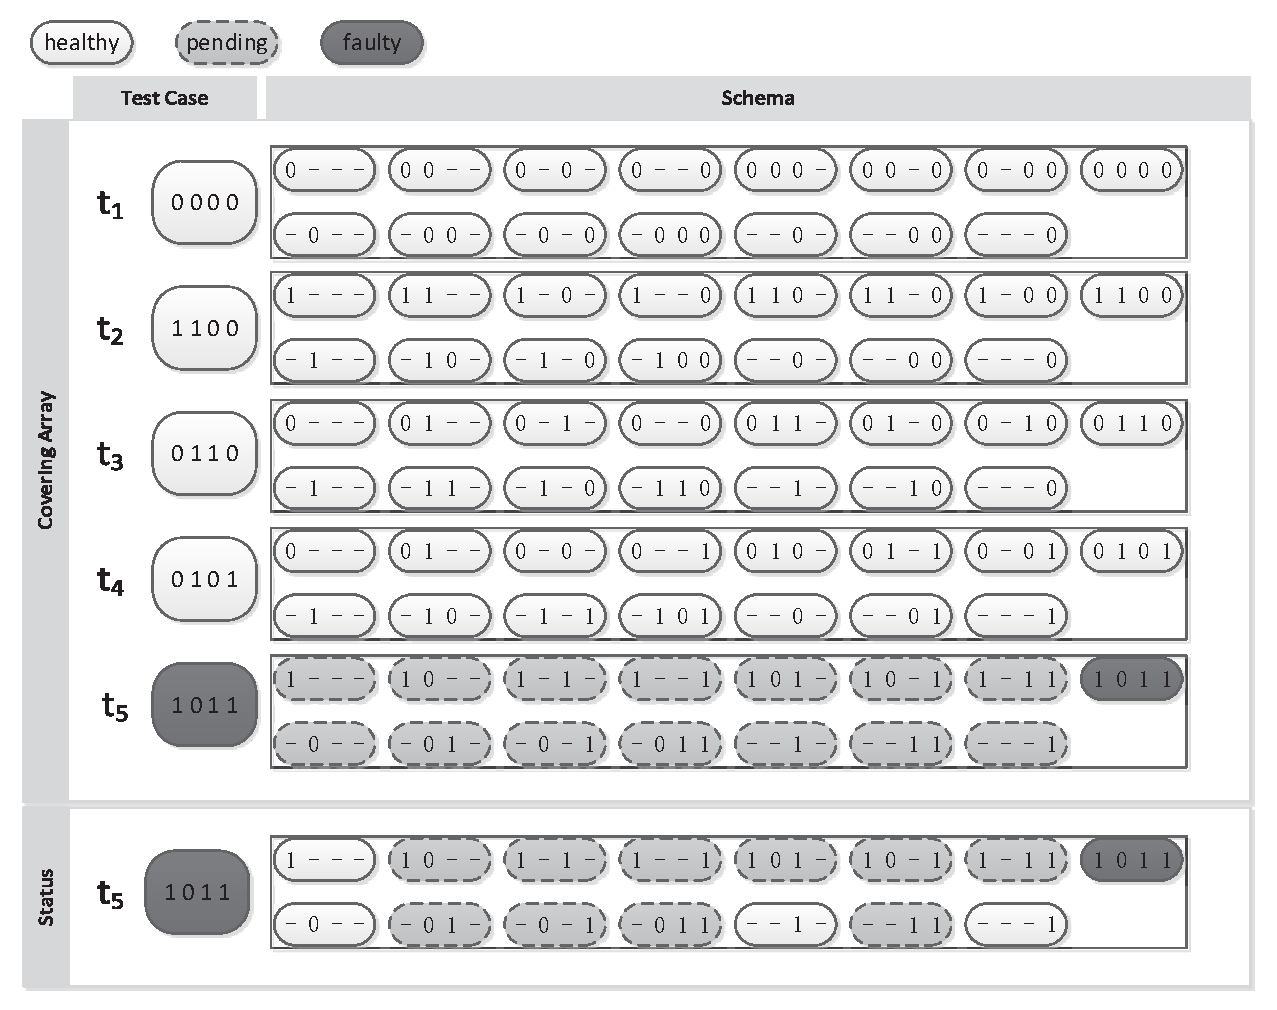
\includegraphics[width=5.6in]{ca.eps}
 \caption{The incompleteness of Covering array }
 \label{fig_inc_ca}
\end{figure*}

In this figure, the test case with dark color represents a failing test case, while the test case with white color is a passing test case. The schema with white color is non-faulty, i.e., will not cause a failure, while the schema with dark color is faulty, i.e., any test case contain this schema would fail after testing. At last, the schema with light dark color and dashed outline is the pending schema, indicating that we cannot still determine whether it is faulty or non-faulty.

In this figure, we can first observe that all the schemas in the passing test case is non-faulty. This result is according to the first rule we mentioned before. The second observation is that the schema with the maximal number of factors (4 factors) in a failing test case is a faulty schema. In fact, this schema is the failing test case itself, i.e., (1, 1, 0, 1). This is because the failing test case must contain at least one MFS (otherwise, it will not fail). Hence, the schema which is the test case itself must also contain at least one MFS. As a result, it must be faulty schema according to the second rule we mentioned before. The last observation is that the other schemas in this failing test case $t_{5}$ are not guaranteed to be faulty schemas. In fact, if we assume this test case only contains one MFS (1, 1, 0, 1), then all the other schemas can be non-faulty schemas. Hence, these schemas cannot be determined to be faulty or not if we focus on this failing test case alone. As a result, we label these schemas as pending schemas initially.

Combining the three observations, we can further remove some pending schemas in $t_{5}$ by selecting the schemas that have already been appeared in the passing test cases. These schemas are (1, -, -, -), (-, -, 0, -), (-, 1, -, -), and (-, -, -, 0), which are labeled as non-faulty schemas. At last, the determination results of these schemas of $t_{5}$ can be shown in the ``\emph{Status}'' row. Note that except for these schemas that have been determined to be faulty and non-faulty, there still exist some pending schemas we cannot further removed by the original two rules. For example, (1, 0, -, -) didn't appear in any passing test case, and it did not contain any identified MFS. Hence, in this example, a single covering array is incomplete because of the existence of these pending schemas.

%because any schema can be the MFS in this test case. For example, if the test case itself as MFS, then no other schemas in this test case can be faulty schema.
%Initially. The schema with light dark color and dashed outline is the pending schema. These schemas cannot be determined by these two rules in the beginning. For example, schema (0, -, 1, -) is not appear in any passing test case, neither contain not any MFS.
%
%Initial is pending. Combining all the information, it is non-faulty.
%
%and the schema with
%
%In terms of making the failing test case clear. In this figure, which denoted what. what denoted what.

%\subsection{The incompleteness of error locating array}
%Since that , many approaches give a alleviation of how to compute the remaining schemas, which is called the fault localization. Error locating array is one of them. However, this time, we also give .

\subsection{The incompleteness of OFOT}
%SOFOT
Since covering array alone cannot remove all the pending schema in the failing test cases, we need more information to satisfy this target.  According to the second rule, i.e., the schema that contain the MFS is faulty schema, one method to reduce the number of pending schemas is to filter out those schemas which contain the MFS. However, without knowing the specific MFS in prior, we can only guarantee that the failing test case itself is faulty schema (it must contain the MFS). In fact, with the covering array alone, this is what we can only do to utilize the second rule.

Hence, to further reduce the set of pending schemas, we need to identify the MFS in the failing test case. One-Factor-One-Time (OFOT) \cite{nie2011minimal} is one of the most wildly used MFS identification approach. It identifies the MFS by modifying the original failing test case to see whether the modification would break the MFS in it. More specifically, at each time, it modifies one factor of the original failing test case and keeps the remaining factors to be as the same as the original failing test case. By doing this, it generates one new test case at each time. It then tests the newly generated test case. If this newly generated test case passes, it indicates the modified factor break the MFS in the original failing test case, and therefore, the original factor in the failing test case is one factor in the MFS. Otherwise, the original factor in the failing test case is not the factor in the MFS if the newly generated test case fails.
%Note that this conclusion is based on the newly generated MFS will not introduce new MFS, and hence, OFOT may not always obtain the accurate MFS.
%In fact, all the MFS identification approaches suffer from the need some assumptions to identify the MFS,

%which is also what we do in the covering arrays.
% For all we know is that the schemas as the failing test cases itself contain the MFS, others we do not know. Hence, it is important to identify the MFS to further narrow down the set of pending schemas.
Next, let us use OFOT to identify the MFS and help to narrow down the set of pending schemas of $t_{5}$ in the original covering array. First, we assume that there is one MFS (-, -, 1, 1) in failing test case $t_{5}$.  Then OFOT will work as follows: it generates four additional test cases $t_{6}$ to $t_{9}$ as shown in Figure \ref{fig_ofot_single}, respectively, each of which has one factor to be mutated from $t_{5}$.  Since $t_{8}$ and $t_{9}$ passed after testing, the original two factors (-, -, 1, -) and (-, -, -, 1) in $t_{5}$ are two factors in the MFS. The fails of $t_{6}$ and $t_{7}$ shows that there is no other factors in this MFS. Hence, OFOT identified the schema (-, -, 1, 1) as the MFS, which is identical to the schema (-, -, 1, 1) that we set as MFS in prior.

%MFS identification task is to distinguish. The wildly used approach is OFOT.
\begin{figure*}[ht]
 \centering
 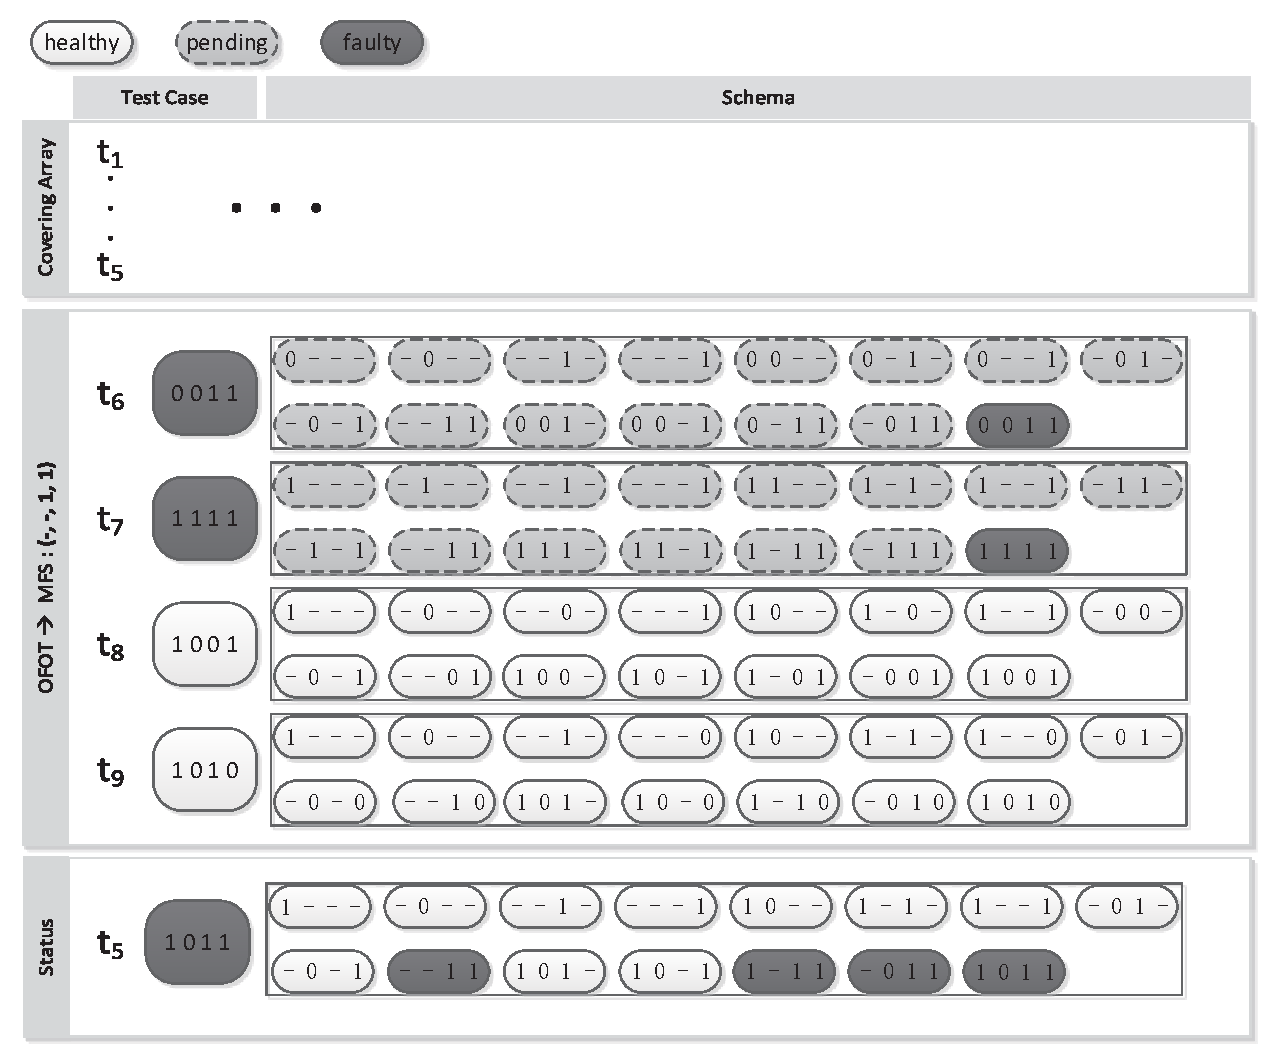
\includegraphics[width=5.6in]{ofot_single.eps}
 \caption{OFOT with single MFS}
 \label{fig_ofot_single}
\end{figure*}

To analyse the pending schemas, we first list all the schemas in each additional test case in Figure \ref{fig_ofot_single}. The same as we observed from the covering array example, for the passing test case $t_{6}$ and $t_{7}$, all the schemas contained in it are non-faulty. For the failing test cases $t_{8}$ and $t_{9}$, we initially set the schemas which are failing test cases themselves as faulty schemas. Other schemas in these two failing test cases are all set to be pending schemas initially.

With these additional information, let us re-consider the status of the schemas in the original failing test case $t_{5}$. Firstly, as the identified MFS is (-, -, 1, 1), we can remove all the pending schemas of $t_{5}$ which contain this schema. These schemas are (-, -, 1, 1), (1, -, 1, 1), (-, 0, 1, 1), and (1, 0, 1, 1), respectively, and are labeled with dark color in the  ``\emph{Status}'' row for $t_{5}$ in Figure \ref{fig_ofot_single}. Next, we remove all the pending schemas of $t_{5}$ which appeared in these two passing test case $t_{6}$ and $t_{7}$. As shown in the  ``\emph{Status}'' row of Figure \ref{fig_ofot_single}, all the remaining pending schemas are removed and labeled with white color. Hence, we can learn that in this single MFS circumstance, OFOT works perfectly to remove all the pending schemas. However, when the failing test case contains multiple MFS, it does not go that well.

Now let us assume there are two MFS in the failing test case $t_{5}$, which are (1, 0, -, -) and (-, -, 1, 1), respectively. At this time, OFOT still generates the same four additional test cases, i.e., $t_{6}$ to $t_{9}$,  as shown in Figure \ref{fig_ofot_multi}. But different from the example of single MFS,  all the additional test cases failed at this time. This is because, the strategy of OFOT, i.e., mutating one factor at one time, cannot break all the MFS at the same time. As a result, it cannot identify any of the MFS.
%Why minimal failure-causing schema is not effective?
%This example shows that . Because there still existing pending schemas.
\begin{figure*}[ht]
 \centering
 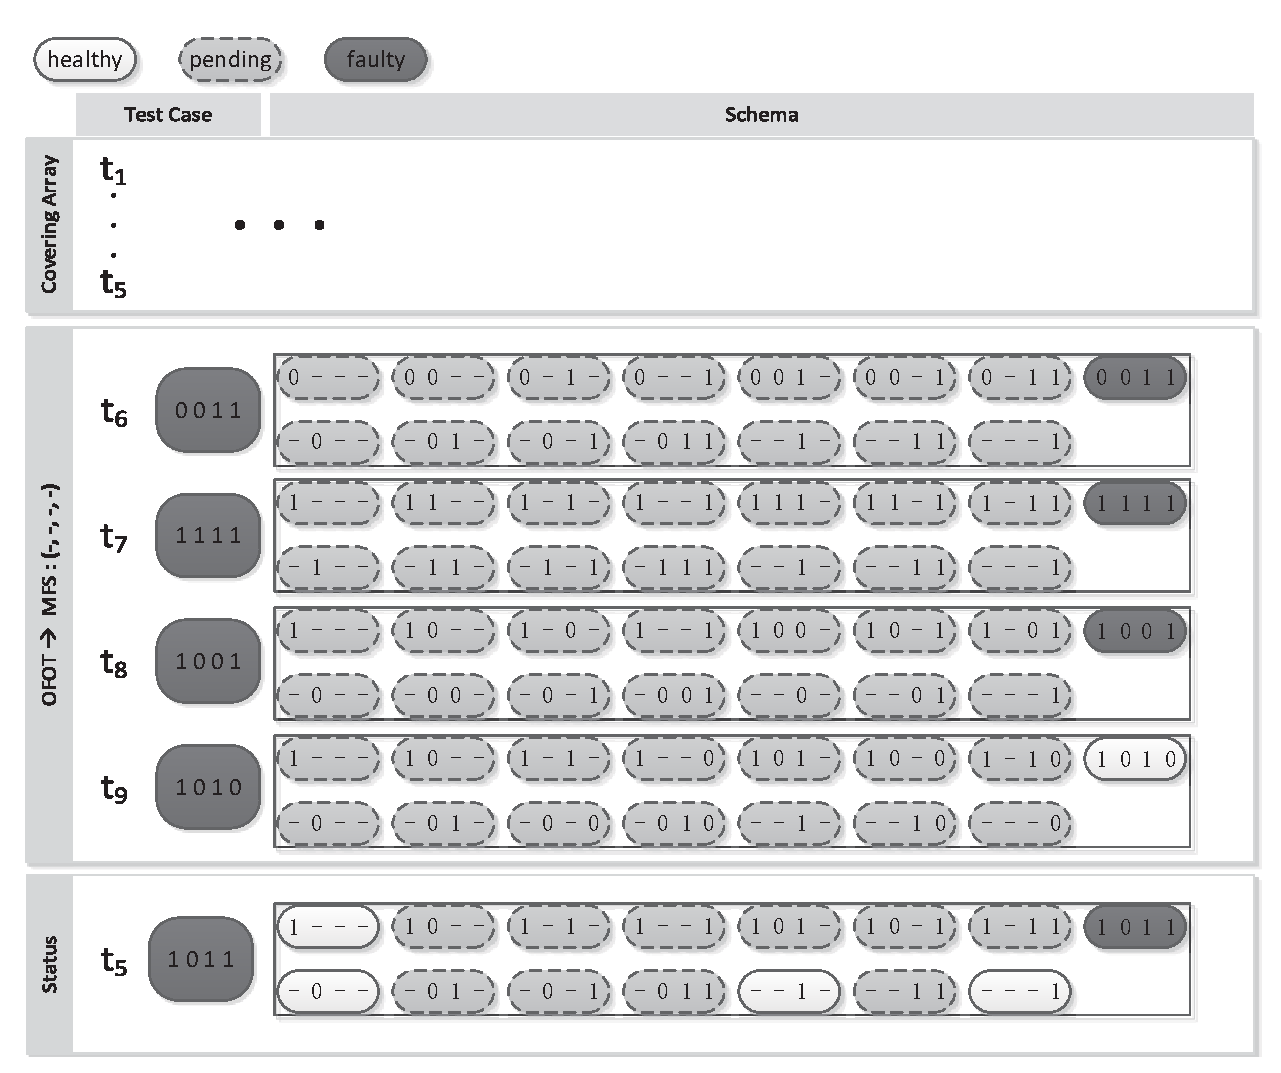
\includegraphics[width=5.6in]{ofot_multi.eps}
 \caption{OFOT with multi MFS}
 \label{fig_ofot_multi}
\end{figure*}

There are two negative influences of this result. First, as we cannot identify the MFS by OFOT, the pending schemas in $t_{5}$ that contain the MFS also cannot be determined. Second, as all the test cases failed after testing, we cannot remove any pending schemas in $t_{5}$ that appear in the passing test case. As a result, the status of the pending schemas of $t_{5}$ will evolve to the ``\emph{Status}'' row of Figure \ref{fig_ofot_single}. We can observe that the status of the schemas of $t_{5}$ is the same as the previous example with only using covering array alone. Hence, in the condition that one failing test case contains multiple MFS, the MFS identification approach OFOT is still incomplete.


\subsection{The incompleteness of FIC}

From the example of OFOT, we can learn the main cause of incompleteness of OFOT is that the failing test case contains multiple MFS. For this, FIC \cite{zhang2011characterizing} (short for Faulty Interaction Characterization) augmented OFOT to handle the multiple MFS problem.
%It also mutates each factor in the original failing test case to generate additional test cases. But different from OFOT, which does not keep the value of the last mutation factor in the next test case generation (at each time, OFOT only mutates one factor and keep the remaining factors the same as the original failing test case), FIC may keep some changes in the next test case generation.  Specifically, when last generated test case failed after testing, FIC will keep the value of the changed factor to the next generations; Otherwise, if the last generated test case passed, FIC will not keep the value of the changed factor and assign the value of the original failing test case to this factor in the next generations. The reason for this is to  make FIC focus on only one MFS at each time and forbidden the appearance of other MFS.
FIC also mutates one factor at a time to generate one additional test case.  The only difference is that it will not always rollback to the original value of one factor it has mutated when it goes on mutating other factors (only when a passing test case appears, it will rollback to the original value). This operation will break multiple MFS in one test case and finally there remains only one MFS to identify. We still use the same example of multiple MFS used in OFOT to illustrate how FIC works and to see whether FIC satisfies the completeness criteria. The result is shown in Figure \ref{fig_fic_multi}.

\begin{figure*}[!htb]
 \centering
 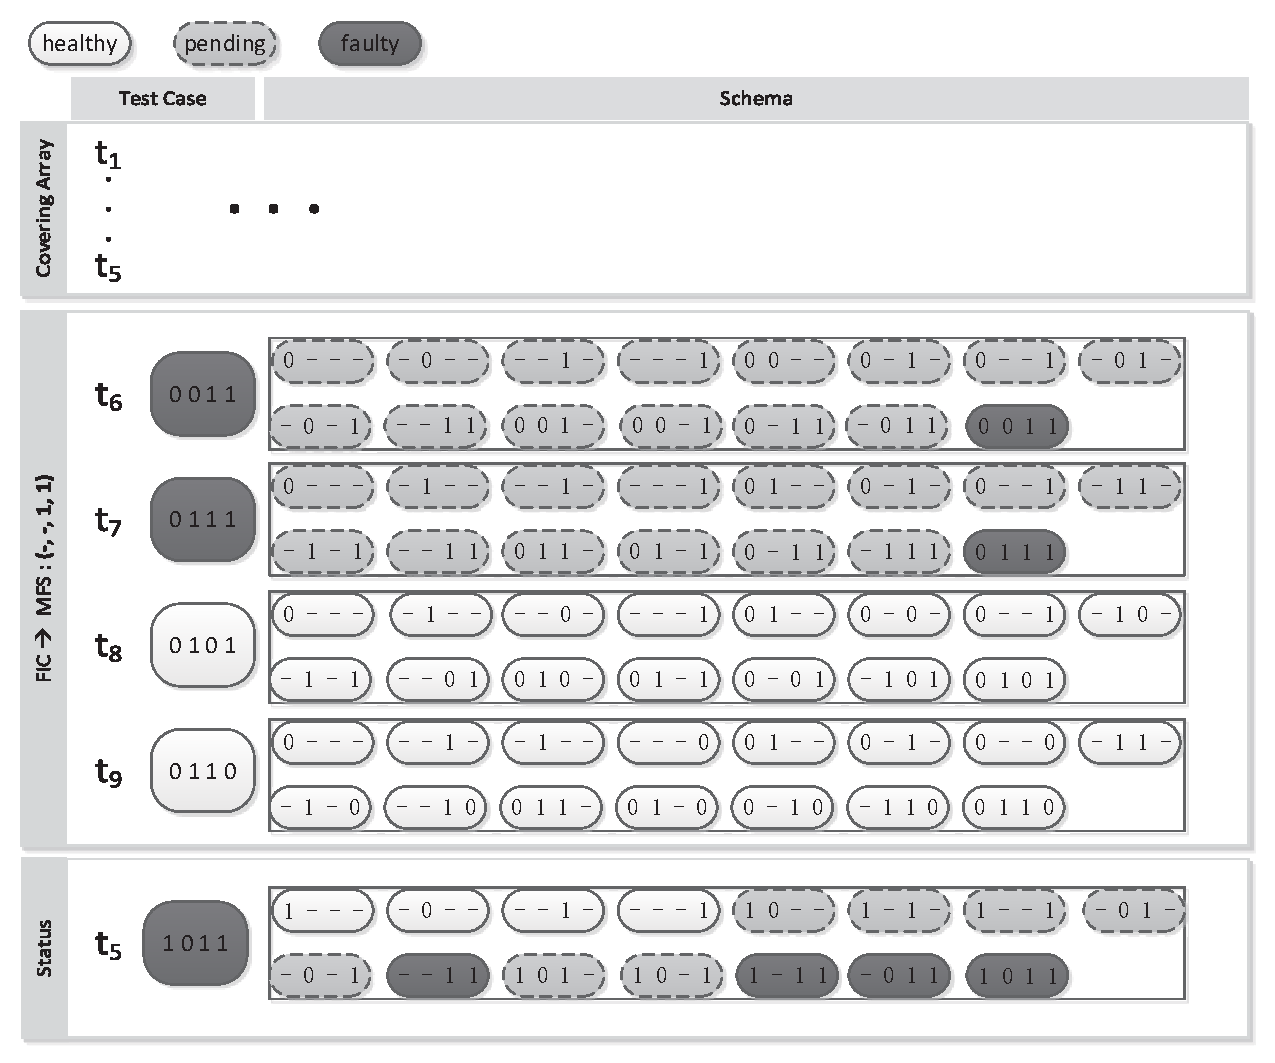
\includegraphics[width=5.3in]{fic.eps}
 \caption{FIC with multiple MFS}
 \label{fig_fic_multi}
\end{figure*}

In Figure \ref{fig_fic_multi}, FIC also generated four additional test cases $t_{6}$ to $t_{9}$. The first case $t_{6}$ is the same as the $t_{6}$ generated by OFOT, but the second additional test case $t_{7}$ generated by FIC is different from $t_{7}$ generated by OFOT. This is because $t_{7}$ generated by FIC keeps the first value of $t_{6}$ (which is a failing test case) instead of the original first value of $t_{5}$. Note that FIC also keeps this value in the following generated test cases $t_{8}$ and $t_{9}$. By doing this, FIC forbids the appearance of the MFS (1, 0, -, -) later. The same as the first value of $t_{6}$, $t_{8}$ and $t_{9}$ keep the second value of $t_{7}$ because $t_{7}$ is also a failing test case. The failings of $t_{6}$ and $t_{7}$ indicated that there still exists other MFS in the original failing test case $t_{5}$, while the first and second factor is not in the remaining MFS.

With respect to the passing test case $t_{8}$, test case $t_{9}$ did not keep the third value of $t_{8}$ but rollback to the value of the original failing test case $t_{5}$. This is because, since $t_{8}$ passed after testing, there is no MFS in this test case. FIC should rollback this value to keep this factor of the MFS and check if there exists other factor of this MFS or not. After all, the passings of $t_{8}$ and $t_{9}$ indicated that (-, -, 1, -) and (-, -, -, 1) are two the factors in the remaining MFS. Hence, the MFS identified by FIC is (-, -, 1, 1).

Next, let us check status of the original failing test case $t_{5}$. The same as OFOT, we first remove the pending schemas that contain the MFS (-, -, 1, 1), and then remove the pending schemas that appear in the additional passing test case. The result is listed in the ``\emph{Status}'' row of Figure \ref{fig_fic_multi}. We can observe that there still exists 6 pending schemas, i.e., (1, 0, -, -), (1, -, 1, -), (1, -, -, 1), (1, 0, 1, -), (1, 0, -, 1), (-, 0, 1, -), and (-, 0, -, 1), respectively.

One reason for this incompleteness that FIC missed anther MFS in the failing test case $t_{5}$, which is (1, 0, -, -). The iterative version of FIC \cite{zhang2011characterizing}, i.e., FINOLP is designed to handle this problem. Specifically, after identifying one MFS in the original failing test case,  FINOLP first generates one more test case by mutating the factors in the original failing test case which appear in the identified MFS. If the generated test case fails after testing, which indicates that there still exists other MFS, it will use FIC to identify the MFS in this generated test case. This process repeats until the test case which is generated by mutating all the factors in the identified MFS passes. Figure \ref{fig_finovlp_multi} shows the detail when applying FINOLP on this example.
%The incompleteness of Finovlp

\begin{figure*}[!htb]
 \centering
 \includegraphics[width=5.3in]{finovlp.eps}
 \caption{FINOVLP with multiple MFS}
 \label{fig_finovlp_multi}
\end{figure*}

In Figure \ref{fig_finovlp_multi}, test cases $t_{1}$ to $t_{9}$ are the same as those of the example in Figure \ref{fig_fic_multi}.  After identifying the MFS (-, -, 1, 1), FINOLP first generated the test case $t_{10}$ to check whether there exists other MFS in the original failing test case $t_{5}$ by mutating the values that appear in this MFS. Since $t_{10}$ failed after testing, it repeated FIC approach on $t_{10}$ to identified the remaining MFS. Therefore, it generated four additional test cases $t_{11}$ to $t_{14}$. The passings of $t_{11}$ and $t_{12}$ indicated another MFS was (1, 0, -, -). FINOLP continued to check whether there exists any other MFS by generating the test case $t_{15}$. The passing of $t_{15}$ showed that there did not exist any other MFS in the original failing test case $t_{5}$. Above all, FINOLP accurately identified all the MFS we have set in piror.

Next, the same as before, we use the two rules to check the status of the pending schemas in the original failing test case $t_{5}$. The result is shown in the ``\emph{Status}'' row of Figure \ref{fig_finovlp_multi}. We can observe that there still exists four schemas, which are (1, -, 1, -), (1, -, -, 1), (-, 0, 1, -), and (-, 0, -, 1), respectively. It is easy to find that these four schemas neither contain any MFS nor appears in any passing test cases. Hence, although FIC and FINOLP can handle the multiple MFS problem, it is still incomplete for the existence of these pending schemas.

\subsection{Additional efforts to remove the pending schemas}

Since Covering array, OFOT, FIC, and FINOLP cannot remove all the pending schemas, more efforts are needed to accomplish this goal. Note that to clear all the pending schemas is important, because some of them can be potential faulty schemas and may be harmful for this system under testing. For this, we decided to check these remaining pending schemas by generating more test cases that contained them and executing these test cases. If these test cases passes, we can directly use the first rule we mentioned before to determine these schemas to be non-faulty schemas. Otherwise, we need to adopt other methods to determine these schemas to be faulty or not.

\begin{figure*}[!htb]
 \centering
 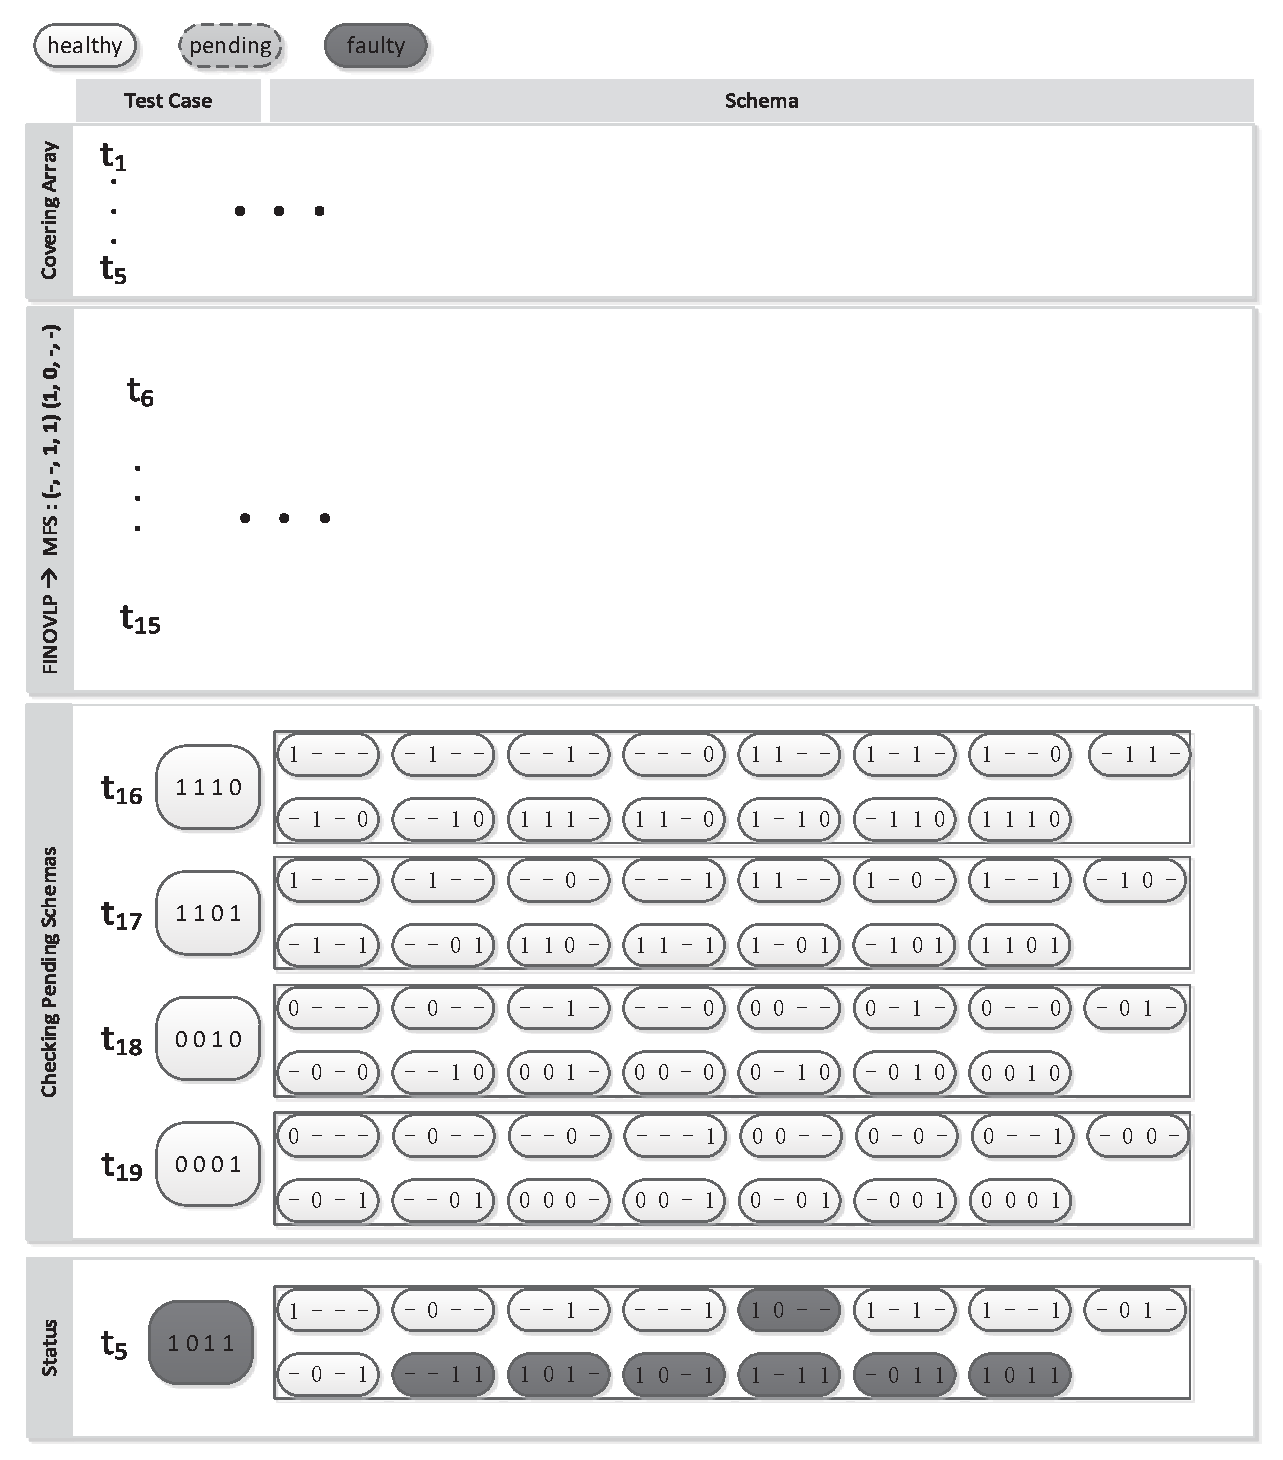
\includegraphics[width=5.3in]{non-pending.eps}
 \caption{Additional efforts to remove pending schemas}
 \label{fig_no_pending}
\end{figure*}

As for this example, we generated four test cases to contain these pending schemas one by one (Note that in this example, we cannot generate one test case contain more than one pending schema without including any MFS). The result is shown in Figure \ref{fig_no_pending}. In this figure, all the additional test cases, i.e., $t_{16}$ to $t_{19}$, passed after testing. Hence, all the remaining schemas are non-faulty schemas. The final status of the pending schemas of $t_{5}$ is shown in the ``\emph{Status}'' row of Figure \ref{fig_no_pending}. We can observe that all the schemas in $t_{5}$ are determined to be non-faulty or faulty. Hence, in this condition, we can guarantee that the test of $t_{5}$ is complete.

Note that if any of the test case ($t_{16}$ to $t_{19}$) failed after testing, we cannot determine whether the corresponding pending schema in that test case is faulty or not.  In this case, we need to generate more test cases to determine the status of this pending schema (If this schema is a faulty schema, the cost will increase exponentially according to the formal definition of faulty schema which will be given later).

\subsection{A summary}

There are two main observations from this section. First, traditional covering array and MFS identification approaches are still incomplete in terms of the existence of pending schemas which cannot be determined to faulty or non-faulty. Second, to remove all the pending schemas is time-consuming. In fact, just listing all the schemas and checking them one by one is inefficient. In this example, we need to check $2^{4} - 15$ schemas for each test case. However, with the increase of the number of factors in one test case, the cost for checking the pending schemas increase exponentially.

For all of these, we need to theoretically analyze the properties of the pending schemas in the failing test cases and to give a more efficient method to obtain them.
%It needs a formal definition and theoretical analysis for the pending schemas with non-faulty schemas and faulty schemas.

\section{Background}\label{sec:back}
This section presents some definitions and propositions to give a formal model for CT.
%\subsection{Failure-inducing interactions in CT}

Assume that the Software Under Test (SUT) is influenced by a set of parameters $P$, which contains \emph{n} parameters, and each parameter $p_{i} \in P$ can take the values from the finite set $V_{i}$ ($i$ = 1,2,..n).

\newtheorem{assumption}{Assumption}
%\newtheorem{proposition}{Proposition}

%\newdef{definition}{Definition}
\begin{definition}\label{de:testcase}
A \emph{test case} of the SUT is a tuple of \emph{n} values, one for each parameter of the SUT. It is denoted as  ($v_{1}$, $v_{2}$,...,$v_{n}$), where $v_{1}\in V_{1}$, $v_{2} \in V_{2}$ ... $v_{n} \in V_{n}$.
\end{definition}
%a \emph{n}-tuple

In practice, these parameters in the test case can represent many factors, such as input variables, run-time options, building options or various combination of them. We need to execute the SUT with these test cases to ensure the correctness of the behaviour of the SUT.

%\begin{definition}
We consider any abnormally executing test case as a \emph{fault}. It can be a thrown exception, compilation error, assertion failure or constraint violation. When faults are triggered by some test cases, it is desired to figure out the cause of these faults.
%Some subsets of these test cases should be analysed.
%\end{definition}


\begin{definition}\label{de:schema}
For the SUT, the $\tau$-set \{$(p_{x_{1}}, v_{x_{1}})$, $(p_{x_{2}}, v_{x_{2}})$, ..., $(p_{x_{\tau}}, v_{x_{\tau}})$\}, where $0 \leq x_{i} \leq n$, $p_{x_{i}} \in P$, and $v_{x_{i}} \in V_{x_{i}}$, is called a $\tau$-degree \emph{schema} ($0 < \tau \leq n $), when a set of $\tau$ values assigned to $\tau$ distinct parameters.
\end{definition}

For example, the interactions (Highlight: Off, Status Bar: On, Smart tags: Off) appearing in Section \ref{sec:intro} is a 3-degree schema, where three parameters are assigned to corresponding values. In effect a test case itself is a n-degree \emph{schema}, which can be described as \{$(p_{1}, v_{1})$, $(p_{2}, v_{2})$, ..., $(p_{n}, v_{n})$\}.

Note that this definition of schema is a formal description of schemas we discussed in the section of \emph{Motivation}. For example, the schema (1, -, 0, -) is exactly the schema \{ $(p_{1}, 1)$, $(p_{3}, 0)$ \} here. We use this formal definition because it benefits the description of the following theoretical analysis, including these propositions and proofs.

\begin{definition}\label{de:subsume}
Let $c_{1}$ be a \emph{l}-degree schema, $c_{2}$ be an \emph{m}-degree schema in SUT and $l \leq m $. If $\forall e \in c_{1}$, $e \in c_{2}$, then $c_{1}$ is the $sub-schema$ of $c_{2}$, and $c_{2}$ the $super-schema$ of $c_{2}$, which can be denoted as $c_{1} \preceq c_{2}$.
\end{definition}

For example,  the 2-degree schema \{(Highlight, Off), (Status Bar, On)\} is a sub-schema of the 3-degree schema \{(Highlight, Off), (Status Bar, On), (Smart tags, Off)\}. Also, since a test case itself is a schema, then if a test case $t$ contains a schema $s$, we have $s \preceq t$. For example,  the 2-degree schema \{(Highlight, Off), (Status Bar, On)\} is also a sub-schema of a test case \{(Highlight, Off), (Status Bar, On), ( Bookmarks, On), (Smart tags, Off)\}

\begin{definition} \label{de:faulty:minimal}
If for any test cases that contain a schema, say $c$, it will trigger a failure, then we call this schema $c$ the \emph{faulty schema}. Additionally, if none of the sub-schema of $c$  except itself is a \emph{faulty schema}, we then call the schema $c$ the \emph{minimal failure-causing schema (MFS)} \cite{nie2011minimal}.

%Based on this, if a test case $t$ hit such a failure-inducing combination, say $c(F)$, it should trigger the fault $F$, for which the test case can be put as $t(F)$
\end{definition}

Note that MFS is identical to the failure-inducing interaction mentioned previously. %In this paper, the terms \emph{failure-inducing interactions} and \emph{MFS} are used interchangeably.
Figuring the MFS helps to identify the root cause of a failure and thus facilitate the debugging process.


\begin{definition}\label{de:healthy:maximal}
A schema, say, $c$, is called a \emph{healthy schema} when we find at least one passing test case that contains this schema. In addition, if none of super-schema of $c$ except itself is the \emph{healthy schema}, we then call the schema $c$ the \emph{maximal healthy schema (MHS)}.
\end{definition}

The healthy schema is exactly the non-faulty schema we mentioned before. These two type of schemas, i.e., MFS and MHS, are essentially representations of the healthy schemas and faulty schemas in a test case. As shown later, other schemas can be determined to be healthy or faulty by these two type of schemas. As a result, we just need to record these two types of schemas (normally a small amount) instead of recording all the schemas in a test case (up to $2^{n}$) when identifying MFS.

%Note that the MFS is based on the assumption that .


%In effect, to identify the MFS in a failing test case is to figure out all the \emph{pending} schemas, and then try to classify each of them into \emph{healthy} or \emph{faulty} schema. After that, the MFS can be selected from those \emph{faulty} schemas by definition.

%\begin{definition}
%If a schema is a \emph{faulty} schema and satisfy the followed condition:
%1. None of its subschemas is \emph{faulty} schema; 2. At least one of its subschemas is \emph{pending} schema. We then call the schema a \emph{candidate minimal faulty schema} (\emph{CMXS}).
%\end{definition}
%
%\begin{definition}
%If a schema is a \emph{healthy} schema and satisfy the followed condition:
%1. None of its super-schemas are healthy schemas; 2. at least one of its subschemas is pending schema. We then call this schema a \emph{candidate maximum healthy schema} (\emph{CMNS}).
%\end{definition}

%Note that failures discussed are assumed to be deterministic in this paper.
To facilitate our discussion, we introduce the following assumptions that will be used throughout this paper:

\begin{assumption}  The execution result of a test case is deterministic.
\end{assumption}

This assumption is a common assumption of CT\cite{zhang2011characterizing,ghandehari2012identifying,niu2013identifying}. It indicates that the outcome of executing a test case is reproducible and will not be affected by some random events. Some approaches have already proposed measures to handle this problem, e.g., studies in \cite{yilmaz2006covering,fouche2009incremental} use multiple covering arrays to avoid this problem.

\begin{assumption} If a test case contains a MFS, it must fail as expected.
\end{assumption}

This assumption shows that we can always observe the failure caused by the MFS. In practice, some issues may prevent this observation. For example, the coincidental correctness problem \cite{Masri:2014:PCC:2582050.2559932} may happen through testing, when the faulty-code is executed but the failure doesn't propagate to the output. Masking effect \cite{yilmaz2013reducing} may also make the failure-observation difficult, as other failure may triggered and stop the program to go on discovering the remaining failures.

We will later discuss the impacts on MFS identification from these two assumptions, as well as how to alleviate them. Based on these definitions and assumptions, we can get several propositions as following. These propositions are the foundations of the theory of pending schemas.
%, and their proofs are omitted due to their simplicity.

\begin{proposition}[Transitive]\label{pro:subsumetrans}
Given schemas $s_{1}$, $s_{2}$, and $s_{3}$, if $s_{1} \preceq s_{2}$, $s_{2} \preceq s_{3}$, then $s_{1} \preceq s_{3}$.
\end{proposition}

This proposition shows the transitivity of the subsuming relationships of schemas, its proof can be directly derived from the definition of the schema.



\begin{proposition}[Sub of Healthy]\label{pro:subofhealthy}
Given a healthy schema $s_{1}$, then $\forall s_{2}, s_{2} \preceq s_{1}$, $s_{2}$ is a healthy schema.
\end{proposition}

\begin{proof}
According to the definition of healthy schema,  there exists at least one test case that contains $s_{1}$ and passes. Let this test case be $t$. Obviously, $s_{1} \preceq t$.  Then $\forall s_{2} \preceq  s_{1}$, we have $s_{2} \preceq s_{1} \preceq t$ according to Proposition \ref{pro:subsumetrans}. Hence, $\forall s_{2} \preceq  s_{1}$,  $t$ contains $s_{2}$ and passes. According to the definition of healthy schema, $\forall s_{2} \preceq  s_{1}$, $s_{2}$ is a healthy schema.
\end{proof}

This proposition shows that any subschema of a healthy schema is also a healthy schema. In fact, this proposition can deduce the first rule in Section \ref{sec:motiv}.


\begin{proposition}[Necessary and sufficient condition to be Healthy]\label{pro:nshealthy}
A schema $s_{1}$ is a healthy schema if and only if $\exists s_{2}, s_{1} \preceq s_{2}$ $\&\&$ $s_{2}$ is a healthy schema.
\end{proposition}

\begin{proof}
Let us first prove the sufficiency. Let $s_{1}$ is a healthy schema. According to the definition, $\exists t$, $s_{1} \preceq t$ and $t$ is a passing test case. In fact, $t$ itself is a schema, and $t \preceq t$, which indicating that $t$ is a healthy schema. Hence, the statement that $\exists s_{2}, s_{1} \preceq s_{2}$ $\&\&$ $s_{2}$ is a healthy schema is true, because $t$ is such a schema.

Then we prove the necessity.  Let $\exists s_{2}, s_{1} \preceq s_{2}$ $\&\&$ $s_{2}$ is a healthy schema be true.  According to Proposition \ref{pro:subofhealthy}, $s_{1}$ is a healthy schema. Hence, the statement $s_{1}$ is a healthy schema is also true.
\end{proof}

This proposition gives necessary and sufficient condition to determine a schema to be healthy or not. Based on this, we can deduce the following lemma.

\begin{lemma}[Non-Healthy]\label{pro:nonhealthy}
A schema $s_{1}$ is not a healthy healthy schema if and only if $\nexists s_{2}, s_{1} \preceq s_{1}$ $\&\&$ $s_{2}$ is a healthy schema.
\end{lemma}

The proof can be directly derived from Proposition \ref{pro:nshealthy}.

%\begin{proposition}[Necessary and sufficient condition to be Healthy]\label{pro:nonsubofhealthy}
%Given a set of healthy schemas $HSS$, we cannot determine a schema, say, $s$, is healthy or not if $\forall s' \in HSS, s \nprec s'$ $\&\&$ $s \neq s'$, i.e., ($s \npreceq s' $).
%\end{proposition}
%
%\begin{proof}
%
%We assume that $s$ is a healthy schema. According to the definition, there exists a passing test case $t$, and $s \prec t$. As $t$ is a passing test case, it is obviously $t \in HSS$.
%
%According to the definition of healthy schema,  there exists at least one test case that contains $s_{1}$ and passes. Let this test case be $t$. Obviously, $s_{1} \prec t$.  Then $\forall s_{2} \prec  s_{1}$, we have $s_{2} \prec s_{1} \prec t$ according to Proposition \ref{pro:subsumetrans}. Hence, $\forall s_{2} \prec  s_{1}$,  $t$ contains $s_{2}$ and passes. According to the definition of healthy schema, $\forall s_{2} \prec  s_{1}$, $s_{2}$ is a healthy schema.
%\end{proof}



\begin{proposition}[Super of Faulty]\label{pro:superoffaulty}
Given a faulty schema $s_{1}$, then $\forall s_{2}, s_{1} \prec s_{2}$, $s_{2}$ is a faulty schema.
\end{proposition}

\begin{proof}
let $T_{2}$ be the set of all the test cases that contain $s_{2}$, we have $\forall t_{2} \in T_{2}$, $s_{2} \prec t_{2}$.  Since $s_{1} \prec s_{2}$, we have $\forall t_{2} \in T_{2}, s_{1} \prec s_{2} \prec t_{2}$ according to the Proposition \ref{pro:subsumetrans}. Hence, $\forall t_{2} \in T_{2}$, $t_{2}$ contains $s_{1}$. According to the definition of faulty schema, any test case which contains $s_{1}$ would fail. Hence, $\forall t_{2} \in T_{2}$, $t_{2}$ is a failing test case. According to the definition of faulty schema. $s_{2}$ is a faulty schema.
\end{proof}

This proposition shows that any super-schema of a faulty schema is also a faulty schema.  Note that his proposition can deduce the second rule in Section \ref{sec:motiv}.


\begin{proposition}[Necessary and sufficient condition to be Faulty]\label{pro:nsfaulty}
A schema $s_{1}$ is a faulty schema if and only if $\exists s_{2}, s_{2} \preceq s_{1}$ $\&\&$ $s_{2}$ is a faulty schema.
\end{proposition}

\begin{proof}
Let us first prove the sufficiency. Let $s_{1}$ is a faulty schema. According to the definition, $\forall t$, $s_{1} \preceq t$ and $t$ is a failing test case. $s_{1}$ itself is a faulty schema.

Then we prove the necessity.  Let $\exists s_{2}, s_{2} \preceq s_{1}$ $\&\&$ $s_{2}$ is a faulty schema be true.  According to Proposition \ref{pro:superoffaulty}, $s_{1}$ is a faulty schema. Hence, the statement $s_{1}$ is a faulty schema is also true.
\end{proof}


\begin{lemma}[Non-Faulty]\label{pro:nonfaulty}
A schema $s_{1}$ is not a faulty schema if and only if $\nexists s_{2}, s_{1} \preceq s_{1}$ $\&\&$ $s_{2}$ is a healthy faulty.
\end{lemma}


%\begin{lemma}[Non-Faulty]\label{pro:nonfaulty}
%Given a set of healthy schemas $HSS$, we cannot determine a schema is healthy or not if $\forall s \in HSS, s_{2} \nprec s_{1}$ $\&\&$ $s_{2} \neq s_{1}$, i.e., ($s_{2} \npreceq s_{1} $).
%\end{lemma}


%You should give normal sentences description and examples of them (if possible, give some simple proofs)

\section{Pending schema}\label{sec:pending}
In this section, we will give the formal definition of the pending schema, as well as its properties. Based on several theoretical analysis about pending schema, we will give an efficient approach to obtain them. Then we will show a case study of  how to apply this approach on identifying the pending schemas.
%To give a better description, we will give several propositions which provide theoretical supports for our approach. The proofs of these propositions are given in the Appendix.



\subsection{What is pending schema}

Through these motivating examples, we can learn that the pending schema is not checked to be healthy and faulty. Hence, we give the definition of the pending schema as follows.


if we find one is pending ? How to depend a pending ?

We first give the formal definition of a schema that cannot be determined to be healthy.
\begin{definition}\label{de:undeteminedhealthy}

\end{definition}

Then, we give the formal definition of  a schema that cannot be determined to be faulty.
\begin{definition}\label{de:undeteminedfaulty}

\end{definition}

\begin{definition}\label{de:pending}
A schema is called a \textbf{\emph{pending} schema}, if it is not yet determined to be \emph{healthy} schema or \emph{faulty} schema.
\end{definition}

The \emph{pending} schema is actually the \emph{cannot-be-determined} schema discussed in Section \ref{sec:intro} and Section \ref{sec:motiv}, which is the key schema we focus on in this paper. To analyse the pending schemas in one failing test case is important to evaluate the completeness of the test.  Next, we will give the first property about the pending schema.
%However, to emulate all the faulty schemas and all the healthy schemas is very large. By the propostios 3 and 4,
%
%More formally, we can learn that it should not be any super-schemas of existing faulty schemas, and any sub-shemas of existing healthy schemas.


\begin{proposition}[Sandwich rule]\label{pro:pending}
Given two pending schemas $s_{1}$, $s_{2}$, and $s_{1} \prec s_{2}$. Then $\forall s_{3}, s_{1} \prec s_{3} \prec s_{2}$, $s_{3}$ is a pending schema.
\end{proposition}

\begin{proof}
We give the proof by contradiction. First, we assume that $s_{3}$ is a faulty schema. Since $s_{3} \prec s_{2}$, then according to Proposition \ref{pro:superoffaulty}, $s_{2}$ is also a faulty schema. This is contradiction as $s_{2}$ is a pending schema. Hence, $s_{3}$ is not a faulty schema. Next, we assume that $s_{3}$ is a healthy schema.  Since $s_{1} \prec s_{3}$, then according to Proposition \ref{pro:subofhealthy}, $s_{1}$ is also a healthy schema. This is also contradiction as $s_{1}$ is a pending schema.  Hence, $s_{3}$ is not a healthy schema. At last, according to the definition of pending schema, $s_{3}$ is a pending schema.
\end{proof}

This proposition gives the determination of pending schemas in the presence of two subsuming pending schemas.

\subsection{Obtaining the pending schemas in a failing test case}
% in a failing test case
Before we give specific method of how to obtain the pending schema, we should first formulate the problem of obtaining schema. Only by doing this can let our approach be general and independent on specific covering arrays or MFS identification approaches. From the motivation example, we can learn that the information offered by covering arrays and MFS identification are a set of healthy schemas (including the passing test case) and faulty schemas (including the failing test case). Based on these information alone, we can obtain the pending schemas in one specific failing test case. Hence, we actually face such a problem that to obtain the pending schema in failing test case in the presence of a set of healthy schemas and faulty schemas.

%Without loss of generality, we assume that .  Note that this formal is to remove the influnce of tests and MFS identification approaches, these just give schemas of which are healthy schemas and faulty schemas.
%
%%To identify the MFS in a failing test case, we need to figure out all the pending schemas and then classify them into faulty or healthy schemas. For this, we firstly need to be able to find one pending schema and check it. Then, we repeat this procedure until no more pending schema can be obtained.
%%first describe how to obtain one pending schema.

Formally, the problem can be defined as follows:

\emph{Given a failing test case $t$ =\{$(p_{1}, v_{1})$, $(p_{2}, v_{2})$, ..., $(p_{n}, v_{n})$\}, a set of faulty schemas $FSS$ = \{ $c_{1}, c_{2}, ... c_{i}, ...$ \},  a set of healthy schemas $HSS$ = \{ $c_{1}, c_{2}, ... c_{i}, ...$ \}, and $FSS \bigcap HSS = \emptyset$. The goal is to find the set of pending schemas, PSS, where $\forall s \in PSS, s \prec t$.}


%\emph{Given a failing test case $t$ =\{$(p_{1}, v_{1})$, $(p_{2}, v_{2})$, ..., $(p_{n}, v_{n})$\}, a set of faulty schemas $FSS$ = \{ $c_{1}, c_{2}, ... c_{i}, ...$ \}, where  $c_{i} \prec t$ or $c_{i} = t$ (That is, $c_{i} \preceq t $), a set of healthy schemas $HSS$ = \{ $c_{1}, c_{2}, ... c_{i}, ...$ \}, where  $c_{i} \preceq t$, and $FSS \bigcap HSS = \emptyset$. The goal is to find one pending schema.}

%Note that at the beginning of MFS identification, if there is no additional information, $FSS$ will be initialized to have one element, i.e., $t$ itself, and $HSS$ is an empty set.

We will settle this problem step by step. According to the Propositions \ref{pro:subofhealthy}. $\forall s $, $s \in HSS$ or $\forall s \in HSS, s' \prec s$ is a healthy schema. That is $s \preceq s' in HSS$ is healthy schema. Note that according to these information (We cannot geneate and execute more test cases to obtain more informaiton), we can only dong this. Second, .

 and \ref{pro:superoffaulty}, it is easy to find that, the pending schemas set PSS should be the following set
\begin{equation}
\begin{aligned}\label{eq:pssfirst}
PSS=\{ c | c \prec t\ \&\&\ \forall c_{f} \in FSS,  c_{f} \npreceq c  \ \&\&\  \forall c_{h} \in HSS, c \npreceq c_{h} \} .
\end{aligned}
\end{equation}

\begin{proof}
\end{proof}

To obtain one pending schema, we just need to select one schema which satisfies $ c \in PSS$. However, to directly utilize Formula \ref{eq:pssfirst} is not practical to obtain one pending schema, because in the worst case it needs to check every schema in a test case $t$, of which the complexity is O($2^{n}$). Hence, we need to find another formula which is equivalent to Formula \ref{eq:pssfirst}, but with much lower complexity.

For this purpose, we defined the following two sets, i.e. CMXS and CMNS.

\begin{definition}
For a k-degree faulty schema c = \{$(p_{x_{1}}, v_{x_{1}})$, $(p_{x_{2}}, v_{x_{2}})$, ..., $(p_{x_{k}}, v_{x_{k}})$\}, a failing test case t = \{$(p_{1}, v_{1})$, $(p_{2}, v_{2})$, ..., $(p_{n}, v_{n})$\}, and $c \preceq t$. We denote the candidate maximal pending schema set as CMXS(c,t)= \{$t \backslash (p_{x_{i}}, v_{x_{i}})$ | $(p_{x_{i}}, v_{x_{i}}) \in c $\}.
\end{definition}

Note that CMXS is the set of schemas that remove one distinct factor value in c, such that all these schemas will not be the super-schema of c. For example assume the failing test case \{$(p_{1}, v_{1})$, $(p_{2}, v_{2})$, $(p_{3}, v_{3})$, $(p_{4}, v_{4})$\}, and a faulty schema \{$(p_{1}, v_{1})$, $(p_{3}, v_{3})$\}. Then the CMXS set is \{ \{$(p_{2}, v_{2})$,  $(p_{3}, v_{3})$, $(p_{4}, v_{4})$\}, \{$(p_{1}, v_{1})$,  $(p_{2}, v_{2})$, $(p_{4}, v_{4})$\} \}. Obviously, the complexity of obtaining CMXS of one faulty schema is O($\tau$), where $\tau$ is the number of parameter values in this faulty schema, i.e., the degree of this schema.

With respect to the CMXS set of a single faulty schema, we can get the following proposition:


\begin{proposition}[one necessary condition, anti faulty schema]\label{pro:subofCMXS}
Given a faulty schema $c_{1}$, a failing test case $t$, where $c_{1} \preceq t$, we have \{$c\ |\ c \prec t\ \&\&\ c_{1} \npreceq c$\} $=$  \{$ c\ |\ \exists c_{1}' \in CMXS(c_{1}, t)$, $c \preceq c_{1}'$\}.
\end{proposition}

This proposition means that the pending schema must be the sub-schema or equal to the schemas in CMXS, otherwise, it is a faulty schema.

In the equation of Proposition \ref{pro:subofCMXS}, the schemas of the left side, i.e., \{$c\ |\ c \preceq t\ \&\&\ c_{1} \npreceq c$\}, are the sub-schemas of test case $t$, but not the super-schemas of faulty schema $c_{1}$ nor equal to $c_{1}$.  Note that the pending schemas can only appear in this set, because any schema that is not belong to this set is faulty schema according to Proposition \ref{pro:superoffaulty}. The right side set in this equation, i.e., \{$ c\ |\ \exists c_{1}' \in CMXS(c_{1}, t)$, $c \preceq c_{1}'$\}, are schemas which are sub-schemas of or equal to at least one schema in $CMXS(c_{1}, t)$. Proposition \ref{pro:subofCMXS} indicates that these two schema sets are equivalent. As an example, considering a failing test case $t$ -- \{($p_{1}$, 1),($p_{2}$, 1),($p_{3}$, 1),($p_{4}$, 1)\}, and a faulty schema $c_{f}$ --  \{($p_{3}$, 1)\}. Table \ref{examleOfCMXSPro} shows the schema set  \{$c\ |\ c \prec t\ \&\&\ c_{f} \npreceq c$\}, $CMXS(c_{f}, t)$ and \{$ c\ |\ \exists c_{1}' \in CMXS(c_{f}, t)$, $c \preceq c_{1}'$\}.

% Table generated by Excel2LaTeX from sheet 'Sheet3'
\begin{table*}[ht]
  \centering
  \setlength{\tabcolsep}{2pt}
  \caption{An example of Proposition \ref{pro:subofCMXS}}
  {\footnotesize
    \begin{tabular}{|c|c|c|c|}
    \hline
  \textbf{  Test case $\textbf{t}$} & \textbf{ \{$\textbf{c}\ |\ \textbf{c} \prec \textbf{t}\ \&\&\ \textbf{c}_{\textbf{f}} \npreceq \textbf{c}$\} }& \textbf{ CMXS($\textbf{c}_{\textbf{f}}, $\textbf{t}$ $)} & \textbf{\{$ \textbf{c}\ |\ \exists \textbf{c}_{\textbf{1}}' \in \textbf{CMXS}\textbf{(}\textbf{c}_{\textbf{f}}, \textbf{t}\textbf{)}$, $\textbf{c} \preceq \textbf{c}_{\textbf{1}}'$ \}}\\\hline
    \{($p_{1}$, 1),($p_{2}$, 1),($p_{3}$, 1),($p_{4}$, 1)\}  & \{($p_{1}$, 1),($p_{2}$, 1),($p_{4}$, 1)\} & \{($p_{1}$, 1),($p_{2}$, 1),($p_{4}$, 1)\} & \{($p_{1}$, 1),($p_{2}$, 1),($p_{4}$, 1)\}\\ \cline{1-1}
      \textbf{Faulty schema $\textbf{c}_{\textbf{f}}$}  & \{($p_{1}$, 1),($p_{2}$, 1)\} &  & \{($p_{1}$, 1),($p_{2}$, 1)\} \\\cline{1-1}
     \{($p_{3}$, 1)\}         & \{($p_{1}$, 1),($p_{4}$, 1)\}&  &\{($p_{1}$, 1),($p_{4}$, 1)\}\\
          &       \{($p_{2}$, 1),($p_{4}$, 1)\} &  &\{($p_{2}$, 1), ($p_{4}$, 1)\}\\
          &       \{($p_{1}$, 1)\} &  &\{($p_{1}$, 1)\}\\
          &       \{($p_{2}$, 1)\} &  &\{($p_{2}$, 1)\}\\
          &       \{($p_{4}$, 1)\} &  & \{($p_{4}$, 1)\}\\\hline
    \end{tabular}}%
  \label{examleOfCMXSPro}%
\end{table*}%

%
%We can find that all these schemas can be find at least one. And all the subschemas of the right side are all in the left side. For example, (12) are all the sub-schemas

%when given a faulty schema $c_{1}$ and a failing test case $t$, the pending schemas can only appeared in set \{$c\ |\ \exists c_{1}' \in CMXS(c_{1}, t), c \preceq c_{1}'$\}.

We can extend this conclusion to a set of faulty schemas. For this, we need the following notation: For two faulty schemas $c_{1}$, $c_{2}$, and a failing test case $t$ ($c_{1} \preceq t$, $c_{2} \preceq t$), let $CMXS(c_{1}, t) \bigwedge CMXS(c_{2}, t)  = \{ c\ |\ c = c_{1}' \cap c_{2}',\ where\ c_{1}' \in CMXS(c_{1}, t),\ and\ c_{2}' \in CMXS(c_{2}, t) \}$.

For example, let $t$ = \{$(p_{1},v_{1}), (p_{2}, v_{2}), (p_{3}, v_{3})$\}, $c_{1}$ = \{$(p_{1}$ $, v_{1}), (p_{2}, v_{2})$\}, $c_{2}$ = \{$(p_{2}, v_{2}), (p_{3}, v_{3})$\}. Then we have $CMXS$ $(c_{1}, t)$ = \{ \{$(p_{1}, v_{1}), (p_{3}, v_{3})$\}, \{$(p_{2}, v_{2}), (p_{3}, v_{3})$\} \}, $CMXS(c_{2},$ $ t)$ = \{ \{$(p_{1}, v_{1}), (p_{2}, v_{2})$\}, \{$(p_{1}, v_{1}), (p_{3}, v_{3})$\} \}, and  $CMXS(c_{1},$ $ t) \bigwedge CMXS(c_{2}, t) = \{ \{(p_{1}, v_{1})\},$ $ \{(p_{1}, v_{1}), $ $(p_{3}, v_{3})\}, $ $ \{(p_{2}, v_{2})\}, $ $\{(p_{3}, v_{3})\} \} $. It is easy to know the complexity of obtaining CMXS of two faulty schemas is O($\tau^{2}$), where $\tau$ is the number of parameter values in the faulty schema. Based on this, we denote $CMXS(FSS,t)$ for a set of faulty schemas.

\begin{definition}
Given a failing test case t = \{$(p_{1}, v_{1})$, $(p_{2}, v_{2})$, ..., $(p_{n}, v_{n})$\}, and a set of faulty schemas FSS = \{$c_{1} , c_{2}, ... c_{i}, ...$\}, where $ c_{i} \preceq t$,  we denote the candidate maximal pending schema of this set as CMXS(FSS,t)= $\bigwedge_{c_{i}\in FSS} CMXS(c_{i}, t)$.
\end{definition}

Note to compute the CMXS of a set of faulty schema, we just need to sequentially compute the CMXS of two faulty schemas until the last schema in this set is computed. Hence, the complexity of obtaining CMXS of a set of faulty schema is O($\tau^{|FSS|}$), where |FSS| is the number of faulty schemas in the schema set, and $\tau$ is the degree of the schema. According to Proposition \ref{pro:subofCMXS}, we have:

\begin{proposition}\label{pro:subofCMXSfor2}
Given a failing test case t = \{$(p_{1}, v_{1})$, $(p_{2}, v_{2})$, ..., $(p_{n}, v_{n})$\}, and a set of faulty schemas FSS = \{$c_{1} , c_{2}, ... c_{i}, ...$\}, where $ c_{i} \preceq t$,  we have \{$c\ |\ c \preceq t\ \&\&\ \forall c_{i} \in FSS, c_{i} \npreceq c $\} $=$  \{$ c\ |\ \exists c_{1}' \in CMXS(FSS, t)$, $c \preceq c_{1}'$\}.
\end{proposition}

Proposition \ref{pro:subofCMXSfor2} extends Proposition \ref{pro:subofCMXS} from a single faulty schema to a set of faulty schemas.

As an example, considering a failing test case $t$ -- \{($p_{1}$, 1),($p_{2}$, 1),($p_{3}$, 1),($p_{4}$, 1)\}, and a set of faulty schemas  $FSS$ -- \{ \{($p_{3}$, 1)\},  \{($p_{1}$, 1), ($p_{2}$, 1)\} \}. Table \ref{examleOfCMXSPro2} shows the schema set \{$c\ |\ c \prec t\ \&\&\ \forall c_{i} \in FSS, c_{i} \npreceq c $\}, $CMXS(FSS, t)$ and \{$ c\ |\ \exists c_{1}' \in CMXS(FSS, t)$, $c \preceq c_{1}'$\}.

% Table generated by Excel2LaTeX from sheet 'Sheet3'

\begin{table*}[ht]
  \centering
  \setlength{\tabcolsep}{2pt}
  \caption{An example of Proposition \ref{pro:subofCMXSfor2}}
  {\footnotesize
    \begin{tabular}{|c|c|c|c|}
    \hline
  \textbf{  Test case $\textbf{t}$} & \textbf{ \{$\textbf{c}\ |\ \textbf{c} \prec \textbf{t}\ \&\&\ \forall \textbf{c}_{\textbf{i}} \in FSS, \textbf{c}_{\textbf{i}} \npreceq \textbf{c}$\} }& \textbf{  CMXS(FSS, t)} & \textbf{\{$ \textbf{c}\ |\ \exists \textbf{c}_{\textbf{1}}' \in \textbf{ CMXS(FSS, t)} $ , $\textbf{c} \preceq \textbf{c}_{\textbf{1}}'$ \}}\\\hline
    \{($p_{1}$, 1),($p_{2}$, 1),($p_{3}$, 1),($p_{4}$, 1)\}  & \{($p_{1}$, 1),($p_{4}$, 1)\} & \{($p_{1}$, 1),($p_{4}$, 1)\} & \{($p_{1}$, 1),($p_{4}$, 1)\}\\ \cline{1-1}
      \textbf{Faulty schema set FSS}  & \{($p_{2}$, 1),($p_{4}$, 1)\} &  \{($p_{2}$, 1),($p_{4}$, 1)\} & \{($p_{2}$, 1),($p_{4}$, 1)\} \\\cline{1-1}
     \{($p_{3}$, 1)\}         & \{($p_{1}$, 1)\}&  &\{($p_{1}$, 1)\}\\
     \{($p_{1}$, 1),($p_{2}$, 1)\}  &       \{($p_{2}$, 1)\} &  &\{($p_{2}$, 1)\}\\
          &       \{($p_{4}$, 1)\} &  & \{($p_{4}$, 1)\}\\\hline
    \end{tabular}}%
  \label{examleOfCMXSPro2}%
\end{table*}%
%
%\begin{proof}
%
%\end{proof}
%Based on previous propositions, we can get that the pending schemas can only appeared in set $P_{up}$ = \{$c\ |\ \exists c_{1}' \in CMXS(FSS,t), c \preceq c_{1}'$\}.


Next, we give the definition of \emph{CMNS}.

\begin{definition}
For a k-degree healthy schema c = \{$(p_{x_{1}}, v_{x_{1}})$, $(p_{x_{2}}, v_{x_{2}})$, ..., $(p_{x_{k}}, v_{x_{k}})$\}, a failing test case t = \{$(p_{1}, v_{1})$, $(p_{2}, v_{2})$, ..., $(p_{n}, v_{n})$\}, and $c \prec t$. We denote the candidate minimal pending schema set as CMNS(c,t)=\{$\{(p_{x_{i}}, v_{x_{i}})\}$ | $(p_{x_{i}}, v_{x_{i}}) \in t \backslash c $\}.
\end{definition}

Note that CMNS is the set of schemas that are assigned to one distinct factor value that is not in c, such that all these schemas will not be the sub-schema of c. For example assume the failing test case \{$(p_{1}, v_{1})$, $(p_{2}, v_{2})$, $(p_{3}, v_{3})$, $(p_{4}, v_{4})$\}, and a healthy schema \{$(p_{1}, v_{1})$, $(p_{3}, v_{3})$\}. Then the CMNS set is \{ \{$(p_{2}, v_{2})$\}, \{$(p_{4}, v_{4})$\} \}.  With respect to the CMNS set of a single healthy schema, we can get the following proposition:

\begin{proposition}[another necessary condition]\label{pro:superofCMNS}
Given a healthy schema $c_{1}$, a failing test case $t$, where $c_{1} \prec t$, we have \{$c\ |\ c \prec t\ \&\&\ c \npreceq c_{1}$\} $=$  \{$ c\ |\ c \prec t \  \&\& \ \exists c_{1}' \in CMNS(c_{1}, t)$, $c_{1}' \preceq c$\}.
\end{proposition}

This proposition means that the pending schema must be the super-schema or equal to the schemas in CMNS, otherwise, it is a healthy schema.

In the equation of Proposition \ref{pro:superofCMNS}, the schemas of the left side, i.e., \{$c\ |\ c \preceq t\ \&\&\ c \npreceq c_{1}$\}, are the sub-schemas of test case $t$, but not the sub-schemas of healthy schema $c_{1}$ nor equal to $c_{1}$.  It is obvious that the pending schemas can also only appear in this set, because they cannot be the sub-schema of any healthy schema nor equal to them. The right side set in this equation, i.e.,\{$ c\ |\ c \preceq t \  \&\& \ \exists c_{1}' \in CMNS(c_{1}, t)$, $c_{1}' \preceq c$\}, are sub-schemas of test case $t$, and also are the super-schemas of or equal to at least one schema in $CMXS(c_{1}, t)$. Proposition \ref{pro:superofCMNS} indicates that these two schema sets are equivalent. As an example, considering a failing test case $t$ -- \{($p_{1}$, 1),($p_{2}$, 1),($p_{3}$, 1),($p_{4}$, 1)\}, and a healthy schema $c_{h}$ --  \{($p_{1}$, 1),($p_{2}$, 1),($p_{3}$, 1)\}. Table \ref{examleOfCMNSPro} shows the schema set  \{$c\ |\ c \prec t\ \&\&\ c_{h} \npreceq c$\}, $CMNS(c_{h}, t)$ and {$ c\ |\ c \prec t\ \&\& \ \exists c_{1}' \in CMXS(c_{h}, t)$, $c_{1}' \preceq c$\}.

% Table generated by Excel2LaTeX from sheet 'Sheet3'
\begin{table*}[ht]
  \centering
  \setlength{\tabcolsep}{2pt}
  \caption{An example of Proposition \ref{pro:superofCMNS}}
  {\footnotesize
    \begin{tabular}{|c|c|c|c|}
    \hline
  \textbf{  Test case $\textbf{t}$} & \textbf{ \{$\textbf{c}\ |\ \textbf{c} \prec \textbf{t}\ \&\&\ \textbf{c} \npreceq \textbf{c}_{\textbf{h}}$\} }& \textbf{ CMNS($\textbf{c}_{\textbf{h}}$, $\textbf{t}$)} & \textbf{\{$ \textbf{c}\ |\ \textbf{c} \prec \textbf{t} \ \&\& \ \exists \textbf{c}_{\textbf{1}}' \in \textbf{CMNS}\textbf{(}\textbf{c}_{\textbf{h}}, \textbf{t}\textbf{)}$, $  \textbf{c}_{\textbf{1}}' \preceq \textbf{c}$ \}}\\\hline
    \{($p_{1}$, 1),($p_{2}$, 1),($p_{3}$, 1),($p_{4}$, 1)\}  & \{($p_{4}$, 1)\} & \{($p_{4}$, 1)\} & \{(($p_{4}$, 1)\}\\ \cline{1-1}
      \textbf{Healthy schema $\textbf{c}_{\textbf{h}}$}  & \{($p_{1}$, 1),($p_{4}$, 1)\} &  & \{($p_{1}$, 1),($p_{4}$, 1)\} \\\cline{1-1}
     \{($p_{1}$, 1),($p_{2}$, 1),($p_{3}$, 1)\}         &\{($p_{2}$, 1),($p_{4}$, 1)\}  &  & \{($p_{2}$, 1),($p_{4}$, 1)\}  \\
                         &\{$p_{3}$, 1),($p_{4}$, 1)\}   &  & \{$p_{3}$, 1),($p_{4}$, 1)\}  \\
                         &\{($p_{1}$, 1),($p_{2}$, 1),($p_{4}$, 1)\}   &  & \{($p_{1}$, 1),($p_{2}$, 1),($p_{4}$, 1)\}  \\
                         &\{($p_{1}$, 1),($p_{3}$, 1),($p_{4}$, 1)\}  &  & \{($p_{1}$, 1),($p_{3}$, 1),($p_{4}$, 1)\}  \\
                         &\{($p_{2}$, 1),($p_{3}$, 1),($p_{4}$, 1)\}  &  & \{($p_{2}$, 1),($p_{3}$, 1),($p_{4}$, 1)\}  \\ \hline
    \end{tabular}}%
  \label{examleOfCMNSPro}%
\end{table*}%


Similarly, for two healthy schemas $c_{1}$, $c_{2}$, and a failing test case $t$ ($c_{1} \preceq t$, $c_{2} \preceq t$), let $CMNS(c_{1}, t) \bigvee $ $CMNS(c_{2}, t)  = \{ c\ |\ c = c_{1}' \cup c_{2}',\ where\ c_{1}' \in CMXS(c_{1}, t),\ and\ c_{2}' \in CMXS(c_{2}, t) \}$.

For example, let $t$ = \{$(p_{1},v_{1}), (p_{2}, v_{2}), (p_{3}, v_{3})$\}, $c_{1}$ = \{$(p_{1}$ $, v_{1}), (p_{2}, v_{2})$\}, $c_{2}$ = \{$(p_{2}, v_{2}), (p_{3}, v_{3})$\}. Then we have $CMNS$ $(c_{1}, t)$ = \{ \{$(p_{3}, v_{3})$\} \}, $CMNS(c_{2},$ $ t)$ = \{ \{$(p_{1}, v_{1})$\} \}, and  $CMNS(c_{1},$ $ t) \bigvee CMNS(c_{2}, t) = \{ \{(p_{1}, v_{1}), (p_{3}, v_{3})\} \} $. Based on this, we denote $CMNS(HSS,t)$ for a set of faulty schemas.


\begin{definition}
Given a failing test case t = \{$(p_{1}, v_{1})$, $(p_{2}, $ $v_{2})$, ..., $(p_{n}, v_{n})$\}, and a set of healthy schemas HSS = \{$c_{1} , c_{2},$ $  ...c_{i}, ...$\}, where $ c_{i} \preceq t$, we denote the candidate minimal pending schema of this set as CMNS(HSS,t)= $ $ $\bigvee_{c_{i}\in HSS}$ $ CMNS(c_{i}, t)$.
\end{definition}

Similar to CMXS(FSS,t), the complexity to obtain CMNS(HSS,t) is O($\tau^{|HSS|}$), where |HSS| is the number of healthy schemas in the schema set, and $\tau$ is the degree of the schema. With respect to CMNS(HSS,t), we have:

\begin{proposition}\label{pro:superofCMNS2}
Given a failing test case t = \{$(p_{1}, v_{1})$, $(p_{2}, v_{2})$, ..., $(p_{n}, v_{n})$\}, and a set of healthy schemas HSS = \{$c_{1} , c_{2}, ... c_{i}, ...$\}, where $ c_{i} \preceq t$,  we have \{$c\ |\ c \prec t\ \&\&\ \forall c_{i} \in HSS, c \npreceq c_{i} $\} $=$  \{$ c\ |\ c \prec t \ \&\& \ \exists c_{1}' \in CMNS(HSS, t)$, $c_{1}' \preceq c$\}.
\end{proposition}

Similar to Proposition \ref{pro:subofCMXS} and \ref{pro:subofCMXSfor2},  Proposition \ref{pro:superofCMNS2} extends Proposition \ref{pro:superofCMNS} from a single healthy schema to a set of healthy schemas.

As an example, considering a failing test case $t$ -- \{($p_{1}$, 1),($p_{2}$, 1),($p_{3}$, 1),($p_{4}$, 1)\}, and a set of schema schemas  $HSS$ -- \{ \{($p_{1}$, 1),($p_{2}$, 1),($p_{3}$, 1)\},  \{($p_{3}$, 1),($p_{4}$, 1)\} \}. Table \ref{examleOfCMNSPro2} shows the schema set \{$c\ |\ c \prec t\ \&\&\ \forall c_{i} \in HSS, c \npreceq c_{i} $\}, $CMNS(HSS, t)$ and \{$ c\ |\ c \prec t \ \&\& \ \exists c_{1}' \in CMNS(HSS, t)$, $c_{1}' \preceq c$\}.

% Table generated by Excel2LaTeX from sheet 'Sheet3'

\begin{table*}[ht]
  \centering
  \setlength{\tabcolsep}{1pt}
  \caption{An example of Proposition \ref{pro:superofCMNS2}}
  {\footnotesize
    \begin{tabular}{|c|c|c|c|}
    \hline
  \textbf{  Test case $\textbf{t}$} & \textbf{ \{$\textbf{c}\ |\ \textbf{c} \prec \textbf{t}\ \&\&\ \forall \textbf{c}_{\textbf{i}} \in \textbf{HSS}, \textbf{c} \npreceq \textbf{c}_{\textbf{i}} $\} }& \textbf{  CMNS(HSS, t)} & \textbf{\{$ \textbf{c}\ |\ \textbf{c} \prec \textbf{t} \ \&\& \ \exists \textbf{c}_{\textbf{1}}' \in \textbf{CMNS(HSS, t)}$, $\textbf{c}_{\textbf{1}}' \preceq \textbf{c}$\}}\\\hline
    \{($p_{1}$, 1),($p_{2}$, 1),($p_{3}$, 1),($p_{4}$, 1)\}  & \{($p_{1}$, 1),($p_{4}$, 1)\} & \{($p_{1}$, 1),($p_{4}$, 1)\} & \{($p_{1}$, 1),($p_{4}$, 1)\}\\ \cline{1-1}
      \textbf{Healthy schema set HSS}  & \{($p_{2}$, 1),($p_{4}$, 1)\} & \{($p_{2}$, 1),($p_{4}$, 1)\} & \{($p_{2}$, 1),($p_{4}$, 1)\} \\\cline{1-1}
     \{($p_{1}$, 1),($p_{2}$, 1),($p_{3}$, 1)\}         &\{($p_{1}$, 1),($p_{2}$, 1),($p_{4}$, 1)\}  &  &  \{($p_{1}$, 1),$p_{2}$, 1),($p_{4}$, 1)\}   \\
     \{($p_{3}$, 1),($p_{4}$, 1)\}         &\{($p_{1}$, 1),($p_{3}$, 1),($p_{4}$, 1)\}    &  &  \{($p_{1}$, 1),($p_{3}$, 1),($p_{4}$, 1)\}  \\
                         &\{($p_{2}$, 1),($p_{3}$, 1),($p_{4}$, 1)\}   &  & \{($p_{2}$, 1),($p_{3}$, 1),($p_{4}$, 1)\}   \\ \hline
    \end{tabular}}%
  \label{examleOfCMNSPro2}%
\end{table*}%


Based on Proposition \ref{pro:subofCMXSfor2} and \ref{pro:superofCMNS2}, we can easily learn that \{$c\ |\ c \prec t\ \&\&\ \forall c_{i} \in FSS, c_{i} \npreceq c $\} $\bigcap$ \{$c\ |\ c \prec t\ \&\&\ \forall c_{i} \in HSS, c \npreceq c_{i} $\}  $=$  \{$ c\ |\ \exists c_{1}' \in CMXS(FSS, t)$, $c \preceq c_{1}'$\} $\bigcap$  \{$ c\ |\ c \prec t \ \&\& \ \exists c_{1}' \in CMNS(HSS, t)$, $c_{1}' \preceq c$\}. Considering $\forall c \in $\{$ c\ |\ \exists c_{1}' \in CMXS(FSS, t)$, $c \preceq c_{1}'$\}, $c \prec t$, we can transform the aforementioned formula into the following equation.

\{$c\ |\ c \prec t\ \&\&\ \forall c_{i} \in FSS, c _{i} \npreceq c \&\&\ \forall c_{i} \in HSS, c \npreceq c_{i}  $\} $=$  \{$ c\ |\ \exists c_{1}' \in CMXS(FSS, t)$, $c \preceq c_{1}'$ $\&\&$ $\exists c_{1}' \in CMNS(HSS, t)$, $c_{1}' \preceq c$\} $=$  \{$ c\ |\ \exists c_{1}' \in CMXS(FSS, t), c_{2}' \in CMXS(FSS, t)$, $c_{2}' \preceq c \preceq c_{1}'$ \}.

Note that the leftmost side of this equation is identical to Formula \ref{eq:pssfirst}, hence, we can learn that

%\begin{equation}\label{eq:psssecond}
%\begin{aligned}
%PSS = & \{ c\ |\ \exists c_{1}' \in CMXS(FSS, t), c \preceq c_{1}' \\
%    & \&\& \exists c_{1}' \in CMNS(HSS, t), c_{1}' \preceq c\}.
%\end{aligned}
%%PSS = \{ c\ |\ \exists c_{1}' \in CMNS(HSS, t), c_{1}' \preceq c \&\& \exists c_{1}' \in CMNS(HSS, t), c_{1}' \preceq c\}.
%\end{equation}

%Further

\begin{equation}\label{eq:psssecond}
\begin{aligned}
PSS =  \{ c\ |\ \exists c_{1}' \in CMXS(FSS, t), c_{2}' \in CMNS(HSS, t),  c_{2}' \preceq c \preceq c_{1}' \}.
\end{aligned}
%PSS = \{ c\ |\ \exists c_{1}' \in CMNS(HSS, t), c_{1}' \preceq c \&\& \exists c_{1}' \in CMNS(HSS, t), c_{1}' \preceq c\}.
\end{equation}

According to Formula \ref{eq:psssecond}, the complexity of obtaining one pending schema is O($ \tau^{|FSS|} \times \tau^{|HSS|}$). This is because to obtain one pending schema, we only need to search the schemas in $CMXS(FSS, t)$ and $CMNS(HSS, t)$, of which the complexity are O($\tau^{|FSS|}$) and O($\tau^{|HSS|}$), respectively. Then we need to check each pair of schemas in these two sets, to find whether exists $c_{1} \in CMXS(FSS, t)$, $c_{2} \in CMNS(HSS, t)$, such that $c_{2} \preceq c_{1}$. If so, then both $c_{2}$ and $c_{1}$ satisfy Formula \ref{eq:psssecond}. Furthermore, $\forall c_{3}, c_{2} \preceq c_{3} \preceq c_{1}$, $c_{3}$ also satisfy Formula \ref{eq:psssecond}. Hence, the complexity of obtaining one pending schema is O($\tau^{|FSS|} \times \tau^{|HSS|}$).

In fact, we can further reduce the complexity of obtaining pending schemas. When given a set of schemas $S$, let the minimal schemas as $S^{\bot } = \{ c | c \in S, \nexists c' \in S, c' \prec c \}$ and the maximal schemas as $S^{\top } = \{ c | c \in S, \nexists c' \in S, c \prec c' \}$. Based on this, we can have the following proposition:

\begin{proposition}\label{pro:identicialPending}
Given a failing test case $t$, a set of faulty schemas $FSS$, and a set of healthy schemas $HSS$, we have \{$ c\ |\ \exists c_{1}' \in CMXS(FSS^{\bot}, t)$, $ c_{2}' \in CMNS($ $HSS^{\top}, t)$, $c_{2}' \preceq c \preceq c_{1}'$ \} $=$  \{$ c\ |\ \exists c_{1}' \in CMXS(FSS, t)$, $c_{1}' \in CMNS(HSS, t)$, $c_{2}' \preceq c \preceq c_{1}'$ \}.
\end{proposition}

As an example, consider a failing test case $t = \{(p_{1}, 1),$ $ (p_{2}, 1), (p_{3}, 1), (p_{4}, 1)\}$, the faulty schema set $FSS =$ \{ $\{(p_{1}, $ $1), (p_{2}, 1), (p_{3}, 1)\}$, $\{(p_{1}, 1), (p_{2}, 1)\}$ \}, and the healthy schema set $HSS =$  \{ $\{(p_{2}, 1),$ $(p_{3}, 1),$ $(p_{4}, 1)\}$, $\{(p_{2}, 1), (p_{3}, 1)\}$ \}. It is easy to learn that the minimal faulty schema set $FSS^{\bot} = \{\{(p_{1}, 1), (p_{2}, 1)\}\}$, and the maximal healthy schema set $HSS^{\top}$ $= \{\{ (p_{2}, 1), (p_{3}, 1), (p_{4}, 1) \}\}$.

Fig \ref{fig_minmax} lists all the faulty schemas, healthy schemas, and pending schemas of test case $t$. At the second part, it lists the $CMXS(FSS, t)$, $CMNS(HSS, t)$, and the schema set \{$ c\ |\ \exists c_{1}' \in CMXS(FSS, t)$, $c_{1}' \in CMNS(HSS, t)$, $c_{2}' \preceq c \preceq c_{1}'$ \}. At last it shows $CMXS(FSS^{\bot}, t)$, $CMNS(HSS^{\top}, t)$ and  \{$ c\ |\ \exists c_{1}' \in CMXS(FSS^{\bot}, t)$, $ c_{2}' \in CMNS($ $HSS^{\top}, t)$, $c_{2}' \preceq c \preceq c_{1}'$ \}.

We can learn that these two schema set mentioned in Proposition \ref{pro:identicialPending} are identical in Fig \ref{fig_minmax}, but the schema set based on $CMXS(FSS^{\bot}, t)$, $CMNS(HSS^{\top}, t)$ used much fewer schemas (3 in total) to obtain the result than the schema set based on $CMXS(FSS, t)$, $CMNS(HSS, t)$ (7 in total). Another observation from this figure is that these two schema set are both identical to the pending schemas. It suggests that using CMXS and CMNS can effectively and efficiently to get the pending schemas, when compared to list all the schemas in a test case and find the pending schema one by one according to Formula \ref{eq:pssfirst}.

\begin{figure*}[ht]
 \centering
 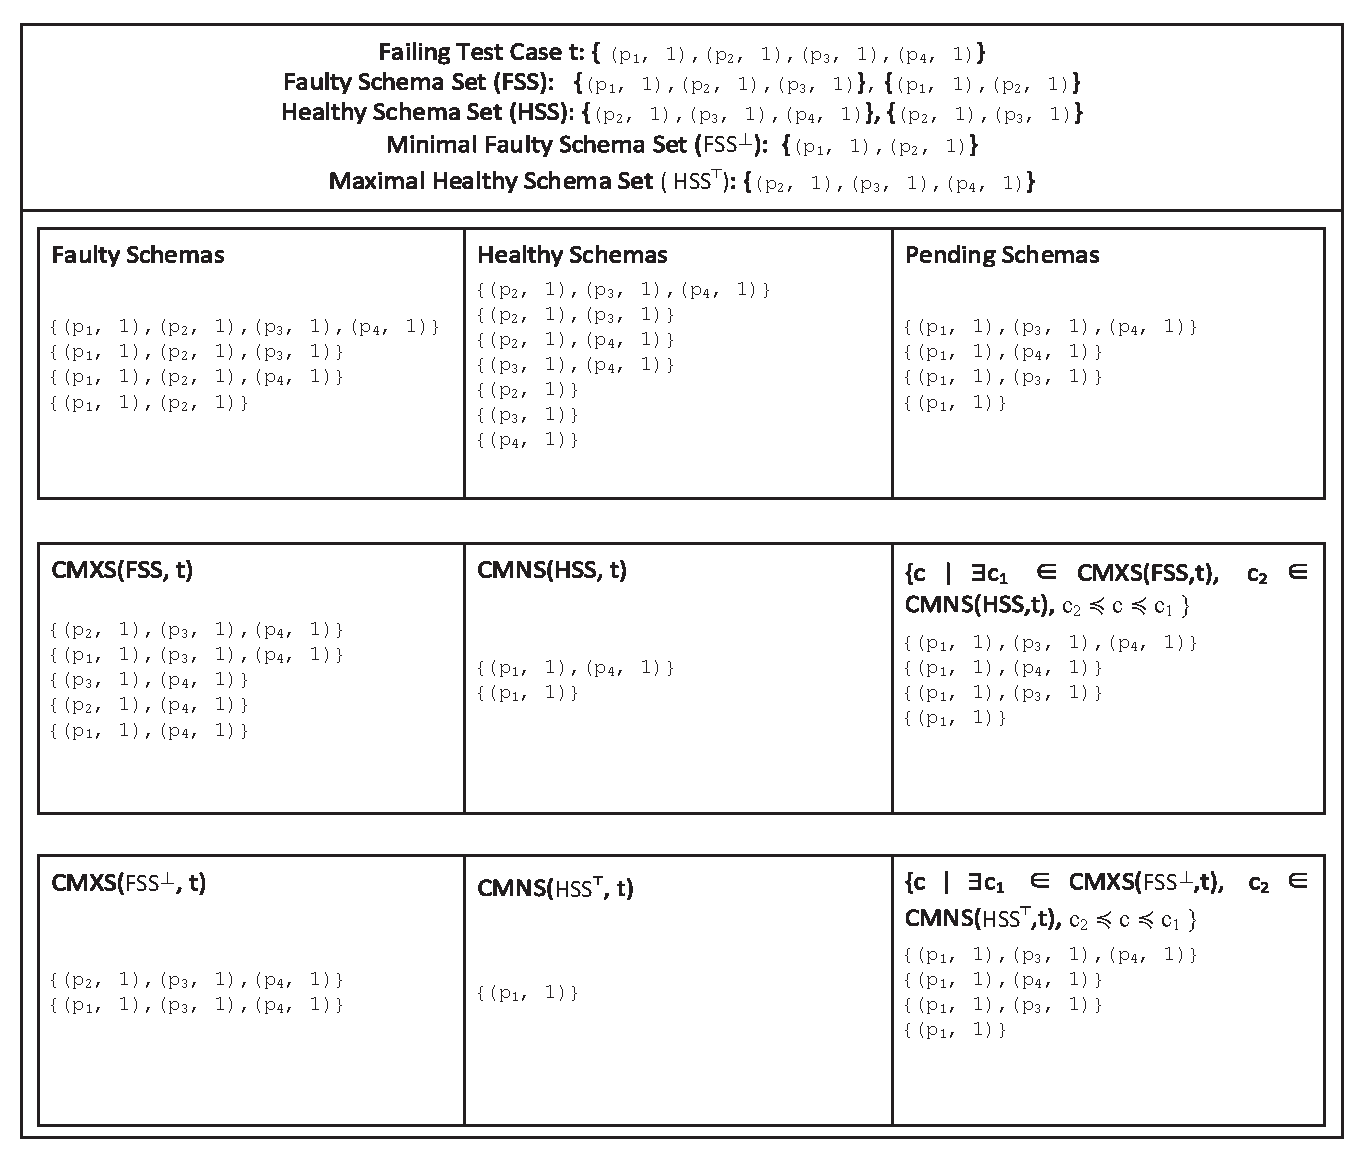
\includegraphics[width=5.6in]{minmax.eps}
 \caption{The example of Proposition \ref{pro:identicialPending}}
 \label{fig_minmax}
\end{figure*}


At last, according to Proposition \ref{pro:identicialPending}, we have the third formula to compute pending schemas as follow:

\begin{equation}\label{eq:pssthird}
\begin{aligned}
PSS =  \{ c\ |\ \exists c_{1}' \in CMXS(FSS^{\bot}, t), c_{2}' \in CMNS(HSS^{\top}, t), c_{2}' \preceq c \preceq c_{1}' \}.
\end{aligned}
%PSS = \{ c\ |\ \exists c_{1}' \in CMNS(HSS, t), c_{1}' \preceq c \&\& \exists c_{1}' \in CMNS(HSS, t), c_{1}' \preceq c\}.
\end{equation}

According to Formula \ref{eq:pssthird}, the complexity of obtaining one pending schema is O($ \tau^{|FSS^{\bot}|} \times \tau^{|HSS^{\top}|}$), where $|FSS^{\bot}|$ and $|HSS^{\top}|$ are two relatively small numbers during MFS identification.

\subsection{A case study of applying Formula \ref{eq:pssthird}}
In this section, we will show a case study of how to obtain the pending schemas with Formula \ref{eq:pssthird}. For consistency, we use the example in the Section \ref{sec:motiv}.
  in the FINOLP. Others are shown in the appendix in a similar way.
From Figure , we can learn that the maximal healthy schemas are the passing test cases themselves, which are $t_{1}$ ,..., and $t_{16}$. While the minimal faulty schemas are the MFS  (Other faulty schemas are the super schemas of this one).
Then we can learn that.  Note that we can learn that .
 
When applying this analysis, we can get back to the motivation example.
We do not need list all the schemas, but we can figure out which one is the pending schema (Covering array, OFOT, OFOT with single  MFS, FIC, FIC with multiple )


% Start of "Sample References" section

\section{Empirical studies}\label{sec:emp}


\subsection{The pending schemas for covering arrays}

%subjects (30 existing wildly used)
%
%generation approaches (ipog, aetg, augmented simulating?)

\subsection{The existence of pending schemas for different MFS identification approaches}

%subjects (my , may also used from )
%
%approaches (my)

\subsection{Does the exitentce of pending schemas contain some potential MFS which may be harmful}
In fact, this is the motivation


\subsection{The characteristics of pending schemas with various types of MFS (multiple, overlapped, single, low-high degrees)}

%the same as the captions


\subsection{The effectiveness of the approach}

%three way: (three formulas in the propositions)


\subsection{Threats to validity}


\section{Discussion}\label{sec:discussion}


\section{Related works}\label{sec:related}
Shi and Nie \cite{shi2005software} presented an approach for failure revealing and failure diagnosis in CT , which first tests the SUT with a covering array, then reduces the value schemas contained in the failing test case by eliminating those appearing in the passing test cases. If the failure-causing schema is found in the reduced schema set, failure diagnosis is completed with the identification of the specific input values which caused the failure; otherwise, a further test suite based on SOFOT is developed for each failing test case, and the schema set is then further reduced, until no more faults are found or the fault is located. Based on this work, Wang \cite{wang2010adaptive} proposed an AIFL approach which extended the SOFOT process by adaptively mutating factors in the original failing test cases in each iteration to characterize failure-inducing interactions.

Nie et al. \cite{nie2011minimal} introduced the notion of Minimal Failure-causing Schema(MFS) and proposed the OFOT approach which is an extension of SOFOT that can isolate the MFS in the SUT. This approach mutates one value of that parameter at a time, hence generating a group of additional test cases each time to be executed. Compared with SOFOT, this approach  strengthens the validation of the factor under analysis and can also detect the newly imported faulty interactions.

Delta debugging \cite{zeller2002simplifying} is an adaptive divide-and-conquer approach to locate interaction failure. It is very efficient and has been applied to real software environment. Zhang et al. \cite{zhang2011characterizing} also proposed a similar approach that can efficiently identify the failure-inducing interactions that have no overlapped part. Later, Li \cite{li2012improved} improved the delta-debugging based approach by exploiting useful information in the executed covering array.

Colbourn and McClary \cite{colbourn2008locating} proposed a non-adaptive method. Their approach extends a covering array to the locating array to detect and locate interaction failures. Mart{\'\i}nez \cite{martinez2008algorithms,martinez2009locating} proposed two adaptive algorithms. The first one requires safe value as the assumption and the second one removes this assumption when the number of values of each parameter is equal to 2. Their algorithms focus on identifying faulty tuples that have no more than 2 parameters.

Ghandehari et al. \cite{ghandehari2012identifying} defined the suspiciousness of tuple and suspiciousness of the environment of a tuple. Based on this, they ranked the possible tuples and generated the test configurations. They \cite{ghandehari2013fault} further utilized the test cases generated from the inducing interaction to locate the fault.

Yilmaz \cite{yilmaz2006covering} proposed a machine learning method to identify inducing interactions from a combinatorial testing set. They constructed a classification tree to analyze the covering arrays and detect potential faulty interactions. Beside this, Fouch{\'e} \cite{fouche2009incremental} and Shakya \cite{shakya2012isolating} made some improvements in identifying failure-inducing interactions based on Yilmaz's work.

Our previous work \cite{niu2013identifying} proposed an approach that utilizes the tuple relationship tree to isolate the failure-inducing interactions in a failing test case. One novelty of this approach is that it can identify the overlapped faulty interaction. This work also alleviates the problem of introducing new failure-inducing interactions in additional test cases.



\section{Conclusion}\label{sec:conclusion}
To identify the MFS in the SUT is important because it provides additional supports to find the cause of the failure. Although many efforts have been proposed to make the MFS identification approaches more efficient and effective, the existence of pending schemas still make them incomplete, which would be hidden dangers to the software under testing. Hence, to identify these pending schemas is of great importance to reveal such potential risks.

In this paper, we studied the characteristics of the relationships among faulty schemas, healthy schemas, minimal failure-causing schemas, and maximal healthy schemas. The subsuming relationships among them form the basis of the methodology for pending schemas. Particulary, we proposed several propositions to formulate the set of pending schemas and give three equivalent formulas to obtain them. Among the three formulas, the last formula reduce the complexity of obtaining pending schemas from O($2^{n}$) to O($ \tau^{|FSS^{\bot}|+|HSS^{\top}|}$), where $n$ is the number of factors in the software, while $|FSS^{\bot}|$ and $|HSS^{\top}|$ are two relatively small numbers and independent on the number of $n$.

We conduct a series empirical studies on some real software systems with various number of parameters and values. Our results shows that the incompleteness in very common in the covering arrays and MFS identification approaches. We also observed that the third proposed formula is the most efficient when compared others in most cases.

As a future work, it is appealing to take the advantages of the pending schemas to assist in the MFS identification approaches. More specifically, we would like to develop a new framework for MFS identification, which take the pending schemas as a indicator. That is, any MFS identification algorithm that runs on this framework aims to empty the set of pending schemas. It is of interest to evaluate the efficiency and effectiveness of this framework with respect to various MFS identification approaches that run on it.

% Appendix
\appendix
\section{Proof}

We will give the proofs of several important propositions.

Proposition \ref{pro:subofCMXS}.
\begin{proof}

Let A =  \{$c\ |\ c \prec t\ \&\&\ c_{1} \npreceq c$\}, and B = \{$ c\ |\ \exists c_{1}' \in CMXS(c_{1}, t)$, $c \preceq c_{1}'$\}.



Let $c_{1}$ = \{$(p_{x_{1}}, v_{x_{1}})$, $(p_{x_{2}}, v_{x_{2}})$, ..., $(p_{x_{k}}, v_{x_{k}})$\},  t = \{$(p_{1}, v_{1})$, $(p_{2}, v_{2})$, ..., $(p_{n}, v_{n})$\}, and CMXS($c_{1}$,$t$)= \{$t \backslash (p_{x_{i}}, v_{x_{i}})$ | $(p_{x_{i}},$ $v_{x_{i}})$ $ \in c_{1} $\}.

First we will show A $\subseteq$ B.

With respect to set A, $\forall c' \in A$, it has $c' \prec t$ and $ c_{1} \npreceq c'$. That is, $\forall e \in c', e \in t$, and  $\exists e' \in c_{1}, e' \not\in c'$. As $c_{1} \preceq t$, $e' \in t$. Hence, we have $\forall e \in c', e \in t \backslash e'$, i.e., $c' \preceq t \backslash e'$.

Since $t \backslash e' \in CMXS(c_{1}, t)$,  $c' \in $ \{$ c\ |\ \exists c_{1}' \in CMXS(c_{1}, t)$, $c \preceq c_{1}'$\} = B. Hence, A $\subseteq$ B.

Second we will show B $\subseteq$ A.

With respect to set B, $\forall c' \in B$, it has $\exists c_{1}' \in CMXS(c_{1}, t), c'$ $ \preceq c_{1}'$. Since $c_{1}' \in CMXS(c_{1}, t)$, $\exists e' \in c_{1}, c_{1}' =  t \backslash e'$. Consequently, $c' \preceq t \backslash e'$. Hence, $c_{1} \npreceq c'$. Also, $c' \preceq t \backslash e' \prec t$. Consequently, $c \in $  \{$c\ |\ c \prec t\ \&\&\ c_{1} \npreceq c$\} = A, which indicates that B $\subseteq$ A.

As we have shown B $\subseteq$ A, and A $\subseteq$ B, so A = B.

\end{proof}

Proposition \ref{pro:subofCMXSfor2}.
\begin{proof}

We just need to prove that for two faulty schemas $c_{1}$, $c_{2}$, and a failing test case $t$ ($c_{1} \preceq t$, $c_{2} \preceq t$), we have \{$c\ |\ c \prec t\ \&\&\ \forall c_{i} \in \{c_{1}, c_{2}\}, c_{i} \npreceq c $\} $=$  \{$ c\ |\ \exists c_{1}' \in CMXS(c_{1}, t)$ $\bigwedge CMXS(c_{2}, t)$, $c \preceq c_{1}'$\}.

Let $A = $ \{$c\ |\ c \prec t\ \&\&\ \forall c_{i} \in \{c_{1}, c_{2}\}, c_{i} \npreceq c $\}, $A_{1}$ = \{$c\ |\ c \prec t\ \&\&\  c_{1} \npreceq c $\}, $A_{2}$ = \{$c\ |\ c \prec t\ \&\&\  c_{2} \npreceq c $\}. It is easily to get $A = A_{1} \bigcap A_{2}$.

Let $B = $ \{$ c\ |\ \exists c_{1}' \in CMXS(c_{1}, t)$ $\bigwedge CMXS(c_{2}, t)$, $c \preceq c_{1}'$\}. Here,  $ CMXS(c_{1}, t) \bigwedge CMXS(c_{2}, t) = \{ c\ |\ c = c_{1}' \cap c_{2}',\ where\ c_{1}' \in CMXS(c_{1}, t),\ and\ c_{2}' \in CMXS(c_{2}, t) \}$.

Let $B_{1} = $ \{$ c\ |\ \exists c_{1}' \in CMXS(c_{1}, t)$, $c \preceq c_{1}'$\}, and $B_{2} = $ \{$ c\ |\ \exists c_{2}' \in CMXS(c_{2}, t)$, $c \preceq c_{2}'$\}. $B_{1} \bigcap B_{2} = $ \{$ c\ |\ \exists c_{1}' \in CMXS(c_{1}, t)$, $c \preceq c_{1}'$ \&\& $\exists c_{2}' \in CMXS(c_{2}, t)$, $c \preceq c_{2}'$\}. Note that, $c \preceq c_{1}'$ \&\& $c \preceq c_{2}'$ $\equiv$ $c \preceq c_{1}' \cap c_{2}'$. Hence, $B_{1} \bigcap B_{2} = $ \{$ c\ |\ \exists c_{1}', c_{2}',\  c_{1}' \in CMXS(c_{1}, t)$, and $c_{2}' \in CMXS(c_{2}, t)$, $c \preceq c_{1}' \cap c_{2}'$ \} = B.

Based on Proposition \ref{pro:subofCMXS}, $A_{1} = B_{1}$, $A_{2} = B_{2}$. Consequently,
$A = A_{1} \bigcap A_{2}$ = $B_{1} \bigcap B_{2}$  = B.

\end{proof}

Proposition \ref{pro:superofCMNS}.

%Given a healthy schema $c_{1}$, a failing test case $t$, we have \{$c\ |\ c \preceq t\ \&\&\ c \npreceq c_{1}$\} $=$  \{$ c\ |\ \exists c_{1}' \in CMNS(c_{1}, t)$, $c_{1}' \preceq c$\}.

\begin{proof}
Let A = \{$c\ |\ c \prec t\ \&\&\ c \npreceq c_{1}$\}. B = \{$ c\ |\ c \prec t \ \&\&\  \exists c_{1}' \in CMNS(c_{1}, t)$, $c_{1}' \preceq c$\}. $CMNS(c_{1},t)$=\{$(p_{x_{i}}, v_{x_{i}})$ | $(p_{x_{i}}, v_{x_{i}}) \in t \backslash c_{1} $\}.

First we will show A $\subseteq$ B.

With respect to set A, $\forall c' \in A$, it has $c' \prec t$ and $c' \npreceq c_{1}$. That is, $\forall e \in c', e \in t$, and  $\exists e' \in c', e' \not\in c_{1}$. Hence, $\{e'\}\ \preceq c',\  e' \in t \backslash c_{1}$, which indicates that $c' \in $ \{$ c\ |\ c \prec t \ \&\&\  \exists c_{1}' \in CMNS(c_{1}, t)$, $c_{1}' \preceq c$\} = B, so A $\subseteq$ B.


Second we will show B $\subseteq$ A.

With respect to set B, $\forall c' \in B$, it has $c' \prec t$  and $\exists c_{1}' \in CMNS(c_{1}, t), c_{1}' \preceq c'$. As $c_{1}' \in CMNS(c_{1}, t)$, $\exists e' \in  t \backslash c_{1}, c_{1}' = \{ e' \}$. Hence, $\{e'\} \preceq c'$. Hence, $c' \npreceq c_{1}$. Consequently, $c' \in $  \{$c\ |\ c \prec t\ \&\&\ c \npreceq c_{1}$\} = A, which indicates that B $\subseteq$ A.

\end{proof}


Proposition \ref{pro:superofCMNS2}.

\begin{proof}
We just need to prove that for two healthy schemas $c_{1}$, $c_{2}$, and a failing test case $t$ ($c_{1} \prec t$, $c_{2} \prec t$), we have \{$c\ |\ c \prec t\ \&\&\ \forall c_{i} \in \{c_{1}, c_{2}\}, c \npreceq c_{i} $\} $=$  \{$ c\ |\ c \prec t \ \&\&\  \exists c_{1}' \in CHFS(c_{1}, t)$ $ \bigvee CHFS(c_{2}, t)$, $c_{1}' \preceq c$\}.

Let $A = $ \{$c\ |\ c \prec t\ \&\&\ \forall c_{i} \in \{c_{1}, c_{2}\}, c \npreceq c_{i} $\}, $A_{1}$ = \{$c\ |\ c \prec t\ \&\&\  c \npreceq c_{1} $\}, $A_{2}$ = \{$c\ |\ c \prec t\ \&\&\  c \npreceq c_{2} $\}. It is easily to get $A = A_{1} \bigcap A_{2}$.

Let $B = $ \{$ c\ |\ c \prec t \ \&\&\  \exists c_{1}' \in CHFS(c_{1}, t)$ $ \bigvee CHFS(c_{2}, t)$, $c \preceq c_{1}'$\}. Here,    $ CMXS(c_{1}, t) \bigvee CMXS(c_{2}, t) = \{ c\ |\ c = c_{1}' \cup c_{2}',\ where\ c_{1}' \in CMXS(c_{1}, t),\ and\ c_{2}' \in CMXS(c_{2}, t) \}$.

Let $B_{1} = $ \{$ c\ |\ c \prec t \ \&\&\  \exists c_{1}' \in CHFS(c_{1}, t)$, $c_{1}' \preceq c$\}, and $B_{2} = $ \{$ c\ |\ c \prec t \ \&\&\  \exists c_{2}' \in CHFS(c_{2}, t)$, $c_{2}' \preceq c$\}. $B_{1} \bigcap B_{2} = $ \{$ c\ |\ c \prec t \ \&\&\  \exists c_{1}' \in CHFS(c_{1}, t)$, $c_{1}' \preceq c$ \&\& $\exists c_{2}' \in CHFS(c_{2}, t)$, $c_{2}' \preceq c$\}. Note that, $c_{1}' \preceq c $ \&\& $c_{2}' \preceq c$ $\equiv$ $c_{1}' \cup c_{2}' \preceq c$. Hence, $B_{1} \bigcap B_{2} = $ \{$ c\ |\ c \preceq t \ \&\&\  \exists c_{1}', c_{2}',\  c_{1}' \in CHFS(c_{1}, t)$, and $c_{2}' \in CHFS(c_{2}, t)$, $ c_{1}' \cup c_{2}' \preceq c$ \} = B.

Based on Proposition \ref{pro:superofCMNS}, $A_{1} = B_{1}$, $A_{2} = B_{2}$. Consequently,
$A = A_{1} \bigcap A_{2}$ = $B_{1} \bigcap B_{2}$  = B.


\end{proof}


Proposition \ref{pro:identicialPending}.
%
%Given a failing test case $t$, a set of faulty schemas $FSS$, and a set of healthy schemas $HSS$, we have \{$ c\ |\ \exists c_{1}' \in CMXS(FSS^{\bot}, t)$, $c \preceq c_{1}'$ $\&\&$ $\exists c_{1}' \in CMNS($ $HSS^{\top}, t)$, $c_{1}' \preceq c$\} $=$  \{$ c\ |\ \exists c_{1}' \in CMXS(FSS, t)$, $c \preceq c_{1}'$ $\&\&$ $\exists c_{1}' \in CMNS(HSS, t)$, $c_{1}' \preceq c$\}.

\begin{proof}
Let A = \{$ c\ |\ \exists c_{1}' \in CMXS(FSS^{\bot}, t)$, $c_{2}' \in $ $CMNS$ $(HSS^{\top}, t)$, $c_{2}' \preceq c \preceq c_{1}'$\}.


Let B =  \{$ c\ |\ \exists c_{1}' \in CMXS(FSS, t)$, $c_{2}' \in CMNS($ $HSS, t)$, $c_{2}' \preceq c \preceq c_{1}'$ \}.


Based on Proposition \ref{pro:subofCMXSfor2} and \ref{pro:superofCMNS2}:

A = \{$c\ |\ c \prec t\ \&\&\ \forall c_{i} \in FSS^{\bot}, c _{i} \npreceq c \ \&\&\  \forall c_{i} \in HSS^{\top}, c \npreceq c_{i}  $\}.

B = \{$c\ |\ c \prec t\ \&\&\ \forall c_{i} \in FSS, c _{i} \npreceq c \ \&\&\  \forall c_{i} \in HSS, c \npreceq c_{i}  $\}.


First we will prove B $\subseteq$ A.

As $FSS^{\bot} \subseteq FSS,\ HSS^{\top} \subseteq HSS$, \{ $c\ |\ \forall c_{i} \in FSS, c_{i} \npreceq c $\}  $\subseteq$  \{ $c\ |\ \forall c_{i} \in FSS^{\bot}, c_{i} \npreceq c $\} and \{ $c\ |\ \forall c_{i} \in HSS, c \npreceq c_{i} $\}  $\subseteq$  \{ $c\ |\ \forall c_{i} \in HSS^{\top}, c \npreceq c_{i} $\}. Hence, \{$c\ |\ c \prec t\ \&\&\ \forall c_{i} \in FSS, c _{i} \npreceq c \ \&\&\  \forall c_{i} \in HSS, c \npreceq c_{i}  $\}  $\subseteq$ \{$c\ |\ c \prec t\ \&\&\ \forall c_{i} \in FSS^{\bot}, c _{i} \npreceq c \ \&\&\  \forall c_{i} \in HSS^{\top}, c \npreceq c_{i}  $\}. That is  $B \subseteq A$.

Next we will prove A $\subseteq$ B.

Note that  $\forall c \prec t$, if $\forall c_{i} \in FSS^{\bot}, c_{i} \npreceq c$, it must have $\forall c_{i}' \in FSS, c_{i}' \npreceq c$. Because if not so, then $\exists c_{i}' \in FSS, c_{i}' \preceq c$. As $\exists c_{i} \in FSS^{\bot}, c_{i}' \in FSS, c_{i} \preceq c_{i}'$, hence, $c_{i} \preceq c_{i}' \preceq c$,  which is contradiction.

Similarly, $\forall c \prec t$, if $\forall c_{i} \in HSS^{\top}, c \npreceq c_{i}$, it must have $\forall c_{i}' \in HSS, c \npreceq c_{i}'$. Because if not so, then $\exists c_{i}' \in HSS, c \preceq c_{i}'$. As $\exists c_{i} \in HSS^{\top}, c_{i}' \in HSS, c_{i}' \preceq c_{i}$, hence, $c \preceq c_{i}' \preceq c_{i}$,  which is contradiction.

Combining them, we can get $\forall c' \in $\{$c\ |\ c \prec t\ \&\&\ \forall c_{i} \in FSS^{\bot}, c _{i} \npreceq c \ \&\&\  \forall c_{i} \in HSS^{\top}, c \npreceq c_{i}  $\}, $c' \in $ \{$c\ |\ c \prec t\ \&\&\ \forall c_{i} \in FSS, c _{i} \npreceq c \ \&\&\  \forall c_{i} \in HSS, c \npreceq c_{i}  $\}. That is, A $\subseteq$ B.

As we have shown B $\subseteq$ A, and A $\subseteq$ B, so A = B.
\end{proof}

\section{Other exmaples when applied the pending shemas}




\begin{acks}

The authors would like to thank the anonymous reviewers for their hard work and valuable comments. This work was supported by the National Key Research and Development Plan(No. 2018YFB1003800), National Science Foundation Award CNS-1748109, US Department of Homeland Security(DHS-14-ST-062-001), and US National Institute of Standards and Technologies Award(70NANB15H199).


\end{acks}

% Bibliography
\bibliographystyle{ACM-Reference-Format}
\bibliography{sample-bibliography}
